%%%%%%%%%%%%%%%%%%%%%%%% Title Page %%%%%%%%%%%%%%%%%%%%%%%%
\documentclass[12pt, a4paper, titlepage]{article}
\usepackage[a4paper,left=3.0cm,right=3.0cm,top=2.54cm,bottom=2.54cm]{geometry}

\usepackage{placeins}
\usepackage{float}
\usepackage{hyperref}
\usepackage{graphicx}
\usepackage{appendix}
\usepackage{setspace}
\usepackage{dcolumn}
\usepackage[printonlyused, withpage]{acronym}
\usepackage{amsmath}
\usepackage{xcolor}
\DeclareMathOperator*{\argmax}{arg\,max} 
\usepackage{natbib}
\makeatletter
\newcommand{\MSonehalfspacing}{%
  \setstretch{1.44}%  default
  \ifcase \@ptsize \relax % 10pt
    \setstretch {1.448}%
  \or % 11pt
    \setstretch {1.399}%
  \or % 12pt
    \setstretch {1.433}%
  \fi
}
\newcommand{\MSdoublespacing}{%
  \setstretch {1.92}%  default
  \ifcase \@ptsize \relax % 10pt
    \setstretch {1.936}%
  \or % 11pt
    \setstretch {1.866}%
  \or % 12pt
    \setstretch {1.902}%
  \fi
}
\makeatother
\MSonehalfspacing

\usepackage{listings}
\usepackage{xcolor}

\colorlet{punct}{red!60!black}
\definecolor{background}{HTML}{EEEEEE}
\definecolor{delim}{RGB}{20,105,176}
\colorlet{numb}{magenta!60!black}

\lstdefinelanguage{json}{
    basicstyle=\normalfont\ttfamily,
    numbers=left,
    numberstyle=\scriptsize,
    stepnumber=1,
    numbersep=8pt,
    showstringspaces=false,
    breaklines=true,
    frame=lines,
    backgroundcolor=\color{background},
    literate=
     *{0}{{{\color{numb}0}}}{1}
      {1}{{{\color{numb}1}}}{1}
      {2}{{{\color{numb}2}}}{1}
      {3}{{{\color{numb}3}}}{1}
      {4}{{{\color{numb}4}}}{1}
      {5}{{{\color{numb}5}}}{1}
      {6}{{{\color{numb}6}}}{1}
      {7}{{{\color{numb}7}}}{1}
      {8}{{{\color{numb}8}}}{1}
      {9}{{{\color{numb}9}}}{1}
      {:}{{{\color{punct}{:}}}}{1}
      {,}{{{\color{punct}{,}}}}{1}
      {\{}{{{\color{delim}{\{}}}}{1}
      {\}}{{{\color{delim}{\}}}}}{1}
      {[}{{{\color{delim}{[}}}}{1}
      {]}{{{\color{delim}{]}}}}{1},
}

\usepackage{caption}
\usepackage{subcaption}

%%%%%%%%%%%%%%DOCUMENT%%%%%%%%%%%%%%
\begin{document}
%%%%%%%%%%%%%%TITLEPAGE%%%%%%%%%%%%%%
\begin{titlepage}
    \begin{center}
    {\LARGE \textbf{Job Title Classification Strategies for the German Labor Market}}
    \\[1cm]
    {\Large \textbf{Masterthesis}}
    \\[1cm]
    {\Large submitted by}
    \\[0.5cm]
    {\LARGE \textbf{Rahkakavee Baskaran}}
    \\[0.5cm]
    {\Large at the}
    \\[0.5cm]
    
\includegraphics[width=0.4\textwidth]{logo.jpg}
    \\[1cm]
    {\Large \textbf{Department of Politics and Public Administration}}
    \\[1cm]
    {\Large \textbf{Center for Data and Methods}}
    \\[2cm]
    \begin{minipage}[c]{0.8\textwidth}
    \begin{description}
     \item {\Large \textbf{1.Gutachter:} Prof. Dr. Susumu Shikano}
     \item {\Large \textbf{2.Gutachter:} JunProf Juhi Kulshresthra}
    \end{description}
    \end{minipage}
    \vfill
    {\LARGE \textbf{Konstanz, \today}}
    \end{center}
    \end{titlepage}

%%%%%%%%%%%%%%TableOfContents%%%%%%%%%%%%%%
\tableofcontents
\newpage


%%%%%%%%%%%%%%Abbreviations%%%%%%%%%%%%%%
\section*{Abbreviations}
\begin{acronym}
  \acro{SVM}[SVM]{Support Vector Machine}
  \acro{NB}[NB]{Naive Bayes}
  \acro{MLR}[MLR]{Multinomial Logistic Regression}
  \acro{OA}[OA]{overall accuracy}
  \acro{ROC}[ROC]{receiver operating characteristics}
  \acro{TP}[TP]{True positives}
  \acro{TN}[TN]{True negatives}
  \acro{FN}[FN]{False negatives}
  \acro{FP}[FP]{False positives}
  \acro{MAP}[MAP]{maximum a posteriori}
  \acro{KldB}[KldB]{Klassifikation der Berufe 2010}
  \acro{ISCO}[ISCO]{International Standard Clasification of Occupations}
  \acro{BOW}[BOW]{Bag of Words}
  \acro{TF-IDF}[TF-IDF]{Term Frequency - Inverse Document Frequency}
  \acro{TF}[TF]{Term Frequency}
  \acro{IDF}[IDF]{Inverse Document Frequency}
  \acro{DF}[DF]{Document Frequency}
  \acro{CBOW}[CBOW]{continous bag of words}
  \acro{BERT}[BERT]{Bidirectional Encoder  Representations from Transformers}
  \acro{NLP}[NLP]{Nature Language Processing}
  \acro{PCA}[PCA]{Principal Component Analysis}
  \acro{RF}[RF]{Random Forest}
  \acro{CART}[CART]{Classification and Regression Trees}
  \acro{CNN}[CNN]{Convolutional Neural Network}
  \acro{KNN}[KNN]{K-nearest neighbors}
  \acro{LR}[LR]{Logistic Regression}
  \acro{RNN}[RNN]{Recurrent Neural Networks}
\end{acronym}
\newpage

%%%%%%%%%%%%%%SECTIONS%%%%%%%%%%%%%%
\section{Introduction}
\section{Related work}
\subsection{Textclassification}
Text classification, a highly researched area, is the process of classifying text documents or text segments into a set of predefined classes. During the last decades, researches developed a various number of classifiers. As \cite{kowsari2019text} summarize in their survey of classifiers, we can group the approaches mainly into three groups. The first group contains traditional methods like \ac{NB},\ac{SVM}), \ac{KNN}, \ac{LR} or Decision Trees \citep{Vijayan2017, Colas2006, kowsari2019text, Sebastiani2001}. Deep learning methods like \ac{CNN} or \ac{RNN}, which are currently the most advanced algorithms for NLP, form the second group. The last group consists of ensemble learning techniques like Boosting and Bagging. Each group can be further split mainly into supervised and unsupervised learning techniques. Since labelled data is available for the classificaiton task in this paper, in the following the focus will be on supervised learning techniques. 

Classification algorithms can be selected on different criteria. Certainly one of the most important criteria is performance. Currently deep learning methods often outperform traditional methods and ensemble techniques. Deep Learning methods are advanced methods of traditional machine learning algorithms. In contrast to traditional methods they do not require a substantive understanding for feature extraction since they automatically extract important features. A lot of comparative studies on traditional and embedding techqniues vs. deep learning text classification tasks show the strength of deep learning. \citet{wang2017} compared \ac{SVM} and \ac{KNN} for web text classification against \ac{CNN}. Additionally he trained a combined \ac{CNN} with \ac{SVM} approach. Despite that the latter show the best performance, his results also reveal a better performance of \ac{CNN} over the traditional methods. \citet{hassan2017} also shows that \ac{CNN}, but also \ac{RNN} outperforms traditional methods with bag of words feature extraction. These results are followed by \citet{kamath2018} who examines among others \ac{LR} and \ac{RF}, a ensemble techniques. Furthmore \citet{gonzalez2020} compared the current state-of-the art deep learning model \ac{BERT} with traditional methods using \ac{TF-IDF} feature selection method and shows clear outperformance by \ac{BERT}. Although deep learning models often outperform traditional methods in these comparative studies, not all classifier have constantly good results over all applications. In contrast to traditional methods, deep learning models also usually require millions of data to train an effective model \citep{chauhan2018}. Thus deep learning methods are not necessarily always the right choice. For example, \citet{zhang2015}, conducted experiments on character-level convolutional neural networks and compared them to different traditional models, like bag-of-words or bag-of-ngrams with \ac{TF-IDF} and \ac{LR}. As data source they fall back on news and review datasets of different size. For the smaller and moderate size datasets the traditional methods except of Bag-of-means performed well and some of them outperformed \ac{CNN}. But for bigger datasets \ac{CNN} worked better. Another study from \citet{yan2018} rely on a siamese CNN deep learning approach with few shot learning for short text classification using different Twitter benchmark data. He compared his results to some baseline deep learning methods and traditional methods, among all \ac{SVM}, ensemble techniques and \ac{LR}. Although the siamese CNN outperformed all the other methods clearly the results are also interesting in another way. Some of the traditional methods outperformed the baseline deep learning methods for specific datasets. 

Comparisons of ensemble technique, traditional methods and methods within the traditional methods indicate as well that not all classifications perform for all tasks equally good or poor. A comparative analysis with \ac{MLR}, \ac{RF} and K-nearest neighbor, using \ac{TF-IDF}, for news text classification indicates a good performance of \ac{MLR} and \ac{RF} compared to K-nearest neighbors, wherby \ac{MLR} performed better then \ac{RF} \citep{shah2020}. A study from biomedical classfication shows best performance of SVM among Random Forest, Naive Bayes with TFIDF \citep{danso2014}. 

Although performance is essential, other criteria like the transparency of the algorithm, the interpretability and efficiency in terms of the runtime are not irrelevant. Methods like \ac{NB} or \ac{LR} are much faster than neural networks or \ac{SVM}s. Considering the transparency and the interpretability algorithms like decision tree or \ac{LR} are more intuitively, easier to understand and to interpretate, while deep learning models and \ac{SVM} rely on complexer computations. Especially deep learning lacks from transperancy \citep{maglogiannis2007}. Considering \ac{BERT} although it outperforms usually other machine learning algorithms for text classification, in general `"there are more questions than answers about how BERT works" \citep[853]{rogers2020}. For example it is not well-understood so far, what exactly happens during the fine-tuning process of \ac{BERT} \citep{merchant2020}. However, the main focus of this analysis is on performance. 

In addition to the criteria of the classifier itself, it is also important for the performance with which inputs the classifiers are fed. Texts must be converted into a numerical representation to make them machine-readable \citep{singh2019}. Mainly the numerical vector representations of a text or document can be divided into sparse and dense vectors, also called word embeddings. Sparse vectors, relying on the \ac{BOW} model, are high-dimensional vectors with a lot of zeros, while word embeddings techniques are fixed length representation \citep{almeida2019}. Sparse vectors are for example \ac{TF-IDF} or count vectorizer. Examples for word embedding techniques are word2vec, doc2vec and \ac{BERT}. 

Unsuitable features considerably affect the performance of the classification algorithm \citep{cahyani2021}. The correct selection of a feature extraction technique depends on many factors, like the length of the dataset or the specific domain \citep{arora2021}. Empirically, this is reflected in the diverse and conflicting studies in the literature. Considering the sparse vectors \citep{wendland2021} compared for fake news data \ac{TF-IDF} and count vectorization and found slightly better results with \ac{TF-IDF} while the results of \citet{WangY2017} show no difference between them. Some studies from different domains demonstrate the strength of word2vec comparing to \ac{TF-IDF} \citep{arora2021, rahmawati2016}, while others show opposite results. \citep{zhu2016,cahyani2021}. \citet{shao2018} conlcude that they find no clear picture between \ac{BOW} models and word2vec. Comparing doc2vec and word2vec \citet{lau2016} found in general a good performance of doc2vec. Although the authors admit that the qualitative differences between both techniques is not clear. Both \citet{shao2018} and \citet{WangY2017} obtain the worst results for doc2vec compared to word2vec and \ac{BOW} vectorization techniques. \ac{BERT} shows overall a good performance \citep{gonzalez2020}. However, \citet{miaschi2020} reach in their study the conclusion that word2vec and BERT code similarly for sentence-related linguistic features. 

\subsection{Challenges of job title classification}
\subsubsection*{Domain-specific and multiclass challenge}
Each text classification task presents different challenges. One challenge is that domain-specific problems may arise. There is some work that deals with job classification in the English speaking job market. 
In terms of classifiers, the corresponding work can be categorised into traditional classifiers or deep learning methods. \cite{Zhu2017} for example, use a KNN classifier in combination with document embedding as feature selection strategy. \cite{Javed2015} rely on traditional methods as well, by combining a SVM classifier and a KNN classifier for their job recommendation system. In contrast, the approaches of \cite{Decorte2021}, \cite{WangJ2019} and \cite{Neculoiu2016} are based on Deep Learning methods. From a higher perspective, there is another dividing line between the approaches. As mentioned earlier, job title normalization can be considered as a typical text classification task \citep{WangJ2019, Javed2015, Zhu2017}. \cite{Decorte2021} and \cite{Neculoiu2016}, however, formulate the task as a string representation approach of similar job titles.  

Another challenge of text classification tasks comes with the number of classes. As \cite{Li2004} show in their classification of tissue, multiclass classification is more difficult than binary classification problems. Partly, because most of classification algorithms were designed for binary problems \citep{Aly2005}. Approaches for multiclassification can be grouped into two types. Binary algorithms can handle multiclassification naturally. This is, for example, the case for Regression, DT, SVM, KNN and NV. The second type is the decomposition of the problem into binary classification tasks (for the different subtypes see \cite{Aly2005}). The literature so far does not have a clear answer to solve multiclassification problems. Different approaches, like Boosting \citep{Schapire2000} or CNN \citep{Farooq2017} are applied. It is noticeable, however, that many works use variations of SVM \citep{Guo2015,Tomar2015,Tang2019}.  

\subsection{Short Text classification} 
Besides the domain specific challenges and multiclassfication another important issue is the length of input documents for classification. Job titles are clearly short text with often not more than 50 characters. Short texts suffer from sparseness, few word co-occurrences, missing shared context, noisiness and ambiguity. These attributes makes it on the one side difficult to construct features, which are capture the meaning of the text. On the other side traditional methods are based on word frequency, high word co-occurrence and context, which is why they often fail to achieve high accuracy for short texts \citep{Song2014, WangY2017, WangF2014,  alsmadi2019}. Besides this short texts are also often characterized as having a lot of misspelling and informal writing. In addition applications delivers and processes short texts in real time. The last three attributes of short texts are indeed a problem, e.g. for Twitter data, which is a popular topic for short text data \citep{karimi2013, sriram2010, yan2018}.  However, for the job title classification they play a little or no role, especially compared to the other stated issues, since job postings are usually reviewed and controlled thoroughly before release. Due to this reason in the following only research concerning the first mentioned attributes is considered. 

A popular approach researches propose for short text classification is to introduce additional knowledge im some way to the features to enhance the short texts. Many studies from the field of Twitter analysis show the power of this approach. \citet{karimi2013}, for example, use a bag of words approach for disaster classification of twitter posts. They experiment with different features enriched by additional information. While for example generic features like number of hashtags improved classifaction other information like incident specific features only helped in spefic settings. All in all they use of bag of words with specific features shows quite good performance. Similarly \citet{sriram2010} achieved with as well with thorougly manual extracted features from the short text good performance for twitter short text messages. 

\citep{WangF2014} criticze the bag of words approach for short text classification, since it result in high dimenisonal data. Especially short text this is much more harmful, because they are short and sparse anyway. They propose a `Bag of concept" approach by using a knowledge base. The knowledgebase is used for learning concepts for each category and find a set of relevant concepts for each short text. Following this, \citep{wang2017J} use as well a enriching concept for short text classification. They use a concept vector with the help of a taxonomy knowledgebase which indicates how much a text is related to the concept. Those are merged with the word embeddings and in addition they add character level features.

In general in short text classifcation the question arises whether to represent the features as dense or sparse vectors. In their comparison between tf-idf/counter vectorizer and the dense vectorizer word2vec and doc2vec, \cite{WangY2017} conclude that among the classifiers Naive Bayes, Logisitic Regression and SVM, the sparse vectorizers achieve the highest accuracy. \cite{Chen2019}, conversely, see limitations in sparse representation as it cannot capture the context information. In their work, they integrate sparse and dense representation into a deep neural network with Knowledge powered Attention, which outperform state-of-art deep learning methods, like CNN, for Chinese short texts. 

\citet{sun2012} pursues in contrast to the mentioned approaches a complete different strategy. Instead of enriching the features he focused the features on specific keywords. In order to select the important key words he used \ac{TF-IDF} approaches, some with a clarity function for each word. Using \ac{LR} he get quite good results for his classification.

Instead of feature enrichment according to \citet{Song2014} a lot of literature focuses on feature dimensionality reduction and extraction of semantic relationship methods using for example Latent Dirichlet approaches. % \citep{zeng2018} use topic modeling approach. 

Concerning the classifiers, there is no consensus approach for short text classification. For traditional approaches \cite{WangY2017}'s results indicate that logistic regression and SVM perform best, while KNN seems to achieve best accuracy in \cite{Khamar2013}'s work. \citet{Song2014} proposes  to use ensemble technqiues. In combination with enriched features \citet{Bouaziz2014}, for example, achieve better results as for \ac{LR}. Similar to job title specific work, more recent work prefers deep learning methods, mostly CNN \citep{Chen2019}. 


\subsection{Implications}
From the above discussed literature three consequences are emerging. First appropriate feature selection or vectorization plays a decisive role in the performance. For that reason, I implement several feature extraction techniques covering sparse and dense vectors. For sparse vectors I vectorize the data with count vectorizer and \ac{TF-IDF} vectorizer. Word2vec, Doc2vec and \ac{BERT} embedding built the group of dense vectorization techniques. The discussion of the different techniques will be the first pillar of the comparison. 

Second, relying on one classification does not seem a reasonable option.  Instead experimenting and exploring different traditional, deep learning and ensemble classifiers allows for identifying the best classifier based on the task and the data \citep{maglogiannis2007}. Therefore I use 4 classifier techniques. I fall back to two traditional methods. The literature shows that \ac{SVM} and \ac{MLR} are well compatible with other technqiues, which is why I choose both of them. I also include an ensemble techqniue: \ac{RF}. As a last method I implement a \ac{BERT} classifier since it is the State-of-Art method currently for text classification. The evaluation of different classifications will built the second pillar of the comparision. 

Third as mentioned above the focus of the presented three challenges is on short text classification. The literature on short text classification reveals two points. There are different results on whether sparse or dense techqniques are better suited. Testing different sparse and dense vectorization techniques allows to cover for that point. Second most of the solutions include additional knowledge. Therefore, I use for the training of the dense embedding techqniques additional knowledge from the Taxonomy and compare the results to the models without adding the knowledge, which will build the last pillar of the comparision. 


\section{Job title data and taxonomy}
The training data consists of two data sets. The classes are extracted from the first data set, referred to below as the \ac{KldB} dataset. The \ac{KldB} dataset contains all information of the \ac{KldB} taxonomy. The second dataset, called job title dataset in the following, contains the necessary data from the job titles. In the first part of this chapter a brief explanation about the Taxonomy structure and both datasets is given. The second part contains of a descriptive analysis of the class distribution of the data. 

\subsection{KldB 2010 Taxonomy}
The ``\ac{KldB}" is structured hierarchically with 5 levels. On each level there is a different number of classes. In the following these classes are also referred to as kldb. On level 1 each class has an id of length one with a number from 0 to 9. Table \ref{tab: T3} shows the 10 classes of level 1 with their class names. On level 2, then, each of the 10 classes are divided into one or more subclasses having a class id of length 2 with the first digit indicating the class of level 1 and the second digit the class of level 2. An overview of the all 5 levels with an example of classes is given in table \ref{tab: T2}. Note that the example in table \ref{tab: T2} does not show on level 2 to level 5 all classes. Thus on level 2 there exists also, e.g. the class id 41 with ``Mathematik-, Biologie- Chemie- und Physikberufe", which in turn is divided into other classes on level 3 etc..  With this procedure this ultimatley leads to class ids of length 5 on level 5. An occupation can be classified on every level in the Taxonomy. Considering the classes of the example in table \ref{tab: T2}, the job title ``Java Developer" could  be classified on level 5 to the class 43412. From this id, it is also derivable that the jobtitle belongs, for example, on level 3 to the class ``Sofwareentwicklung" \citep{Bundesagentur2011a, Bundesagentur2011b, Paulus2013}

The \ac{KldB} contains of two dimension. The first dimension, the so-called "Berufsfachlichkeit" structures jobs according to their similarity in knowledge, activties and jobs. This is reflected in the first 4 levels. Considering the again the example from above and the job title "Fullstack PHP-Entwickler" it is reasonable to classify both on level 1 to "Naturwissenschaft, Geografie and Information", because both of them are related to computer science. It also make sense to classifiy them for example to 4341, because both are about sofware development. On level 5, then, a second dimension is introduced. the "Anforderungsniveau". This dimension gives information on the level of requirement for a job and 4 possible requirements. In table \ref{tab: T4} they are summarized. From the class id of job title ``Java Developer", we can see that the job has been assigned to the second requirement level, since the last digit is a 2 \citep{Bundesagentur2011a,Bundesagentur2011b,Paulus2013}


\begin{table}[]
  \resizebox{\textwidth}{!}{%
  \begin{tabular}{cl}
  \hline
  \multicolumn{1}{l}{\textbf{IDs KldB 2010}} & \textbf{Berufsbereich (Level 1)}                                           \\ \hline
  1                                          & Land-, Forst- und Tierwirtschaft und Gartenbau                             \\
  2                                          & Rohstoffgewinnung, Produktion und Fertigung                                \\
  3                                          & Bau, Architektur, Vermessung und Gebäudetechnik                            \\
  4                                          & Naturwissenschaft, Geografie und Informatik                                \\
  5                                          & Verkehr, Logistik, Schutz und Sicherhe                                     \\
  6                                          & Kaufmännische Dienstleistungen, Warenhandel, Vertrieb, Hotel und Tourismus \\
  7                                          & Unternehmensorganisation, Buchhaltung, Recht und Verwaltung                \\
  8                                          & Gesundheit, Soziales, Lehre und Erziehung                                  \\
  9 & Sprach-, Literatur-, Geistes-, Gesellschafts- und Wirtschaftswissenschaften, Medien, Kunst, Kultur und Gestaltung \\
  0                                          & Militär                                                                    \\ \hline
  \end{tabular}%
  }
  \caption{\label{tab: T3} Overview of classes Level 1 - Berufsbereiche (edited after \citep{Bundesagentur2011b})}
  \end{table}

\begin{table}[hb!]
  \center
  \resizebox{\textwidth}{!}{
  \begin{tabular}{llll}
  \hline
  \textbf{Name}      & \textbf{Level} & \textbf{Number of classes} & \textbf{Example}                               \\ \hline
  Berufsbereiche     & 1              & 10                         & 4: Naturwissenschaft, Geografie und Informatik \\
  Berufshauptgruppen & 2 & 37   & 43: Informatik-, Informations- und Kommunikationstechnologieberufe            \\
  Berufsgruppen      & 3              & 144                        & 434: Sofwareentwicklung                        \\
  Berufsuntergruppen & 4              & 700                        & 4341: Berufe in der Sofwareentwicklung         \\
  Berufsgattungen    & 5 & 1286 & 43412: Berufe in der Sofwareenetwicklung - fachlich ausgerichtete Tätigkeiten \\ \hline
  \end{tabular}%
  }
  \caption{\label{tab: T2} Overview of \ac{KldB} (edited after \citep{Bundesagentur2011b})}
  \end{table}


\begin{table}[]
  \resizebox{\textwidth}{!}{%
  \begin{tabular}{clll}
  \hline
  \multicolumn{1}{l}{\textbf{Level of requirement}} & \textbf{Class ID} & \textbf{Name long} & \textbf{Name short} \\ \hline
  1 & xxxx1 & Helfer- und Anlerntätigkeit        & Helfer     \\
  2 & xxxx2 & fachlich ausgerichtete Tätigkeiten & Fachkraft  \\
  3 & xxxx3 & komplexe Spezialstentätigkeiten    & Spezialist \\
  4 & xxxx4 & hoch komplexe Tätigkeiten          & Experte    \\ \hline
  \end{tabular}%
  }
  \caption{\label{tab: T4} Overview of Level of requirements on Level 5} (edited after \citep{Bundesagentur2011b})
  \end{table}

With the \ac{KldB} 2010, an useful and information-rich occupational classification was created for Germany that reflects the current trends in the labor market \citep{Paulus2013}. One strength relies in the construction of the \ac{KldB}. Instead of just including expert knowledge into the Taxonomy the developement process is based on systematical consideration of information about occupations, as well as statistical procedures for taxonomy developement. Furthermore, the taxonomy was reviewed qualitatively several times in relation to professions and revised. Considering the expressiveness, the \ac{KldB} has some more benefits. Since the taxonmy is quite recent, it reflects new job classes and market trends very adequately. Further, by including the second dimension, the taxonomy provides a powerful tool to organize job titles into simple requirement classes.  In addition, the taxonomy also distinguishes between managerial, supervisory, and professional employees, which is also valuable information. Finally, the taxonomy also convinces with the possibility to switch to ``\ac{ISCO}" through its IDS and thus to normalize jobs to a global standard \citep{Bundesagentur2011b}.

The \ac{KldB} dataset contains different information related to the structure descriped above. Besides the class label, the level and the title, on level 5 for each kldb some searchwords are given. There are two types of keywords. One is the job titles that match the respective kldb. On the other hand, real search words, with the help of which the associated kldb can be inferred. Therefore, these searchwords are very helpful knowledge for training classificaiton algorithms, because they contain kldb specific words that are also often present in the job titles. The searchwords will be termed additional knowledge in the rest of the work. 
 
\subsection{Job title data}
Job Titles can be scraped from the Federal Employment Agency's job board. Employers must provide additional data for each job posting, including the job title, as well as a main internal documentation code that indicates a class in the \ac{KldB} taxonomy. There is an option to provide alternative documentation codes if more than one KLDB class is being considered. An example snippet of the scraped data is provided in the Appendix \footnote{There are two version of the raw data since the Federal Employement Agency changed during the scraping phase the datastructure. Both version are given in the Appendix.} The documentation code is an internal number of the Federal Employment Agency, which can be uniquely assigned to a \ac{KldB}, which, as already mentioned, is specified in the taxonomy data for each kldb. A snippet of the matched training data with the KLDB labels is given in the appendix.

Initially, in total, the training data set contained of 269788 examples. However, during the training phase, it became clear, that there are problems especially with \ac{SVM} classifier, concerning the running time and memory. Due to limited resources, a sample with the same distribution from the long dataset had to be taken. A sample size of 15000 examples proved to be feasible. Figures \ref{fig: F9} and \ref{fig: F10} show the distribution of the classes in level 1 und level 3 \footnote{The class distribution of the long dataset is given in the Appendix.}. Both figures show the absolute number of examples for each kldb in the respective levels. In figure \ref{fig: F10}  the number of examples is coloured with the belonging kldb level 1 class to give better overview of the 144 kldbs on level 3. In general from both levels it is clear that there is in fact that the data is not distributed equally. For the class distribution if level 1 on Figure \ref{fig: F9} class 1 and class 9 have really few examples, while class 2 has considerably more examples than all other classes. Although the data is imbalanced, all classes have at least some examples in order to get meaningful performance measurements. Note that kldbs with digit 0 are missing. 0 stands for `Militär". Jobs in this category are not normally posted frequently on the Employment Agency Job Board page. At level 3, the uneven distribution is even more apparent.Compared to level 1, the problem is that there are a lot of classes with only one example, which is problematic for obtaining interpretable measurements. This problem will be discussed in the results part. In total 8 classes do not have any examples and thus cannot be trained with the classifier.  


\begin{figure}
  \begin{subfigure}{.5\textwidth}
    \centering
    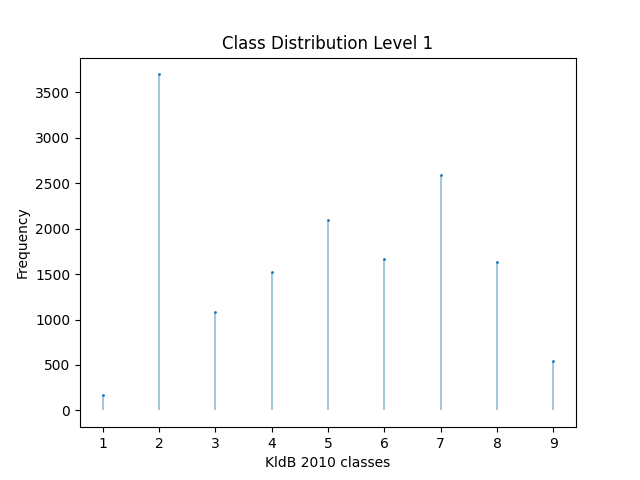
\includegraphics[width=.9\linewidth]{training_data_short_L1.png}
    \caption{\label{fig: F9} Class distribution Level 1}
  \end{subfigure}%
  \begin{subfigure}{.5\textwidth}
    \centering
    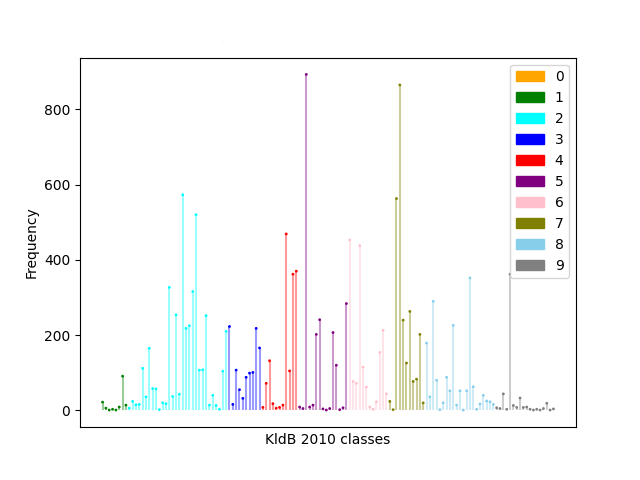
\includegraphics[width=.9\linewidth]{training_data_short_L3.png}
    \caption{\label{fig: F10} Class distribution Level 3}
  \end{subfigure}
  \caption{Class distribution of the training data}
  \end{figure}


\section{Method}
\subsection{Conceptual overview}

\begin{figure}[]
  \center
  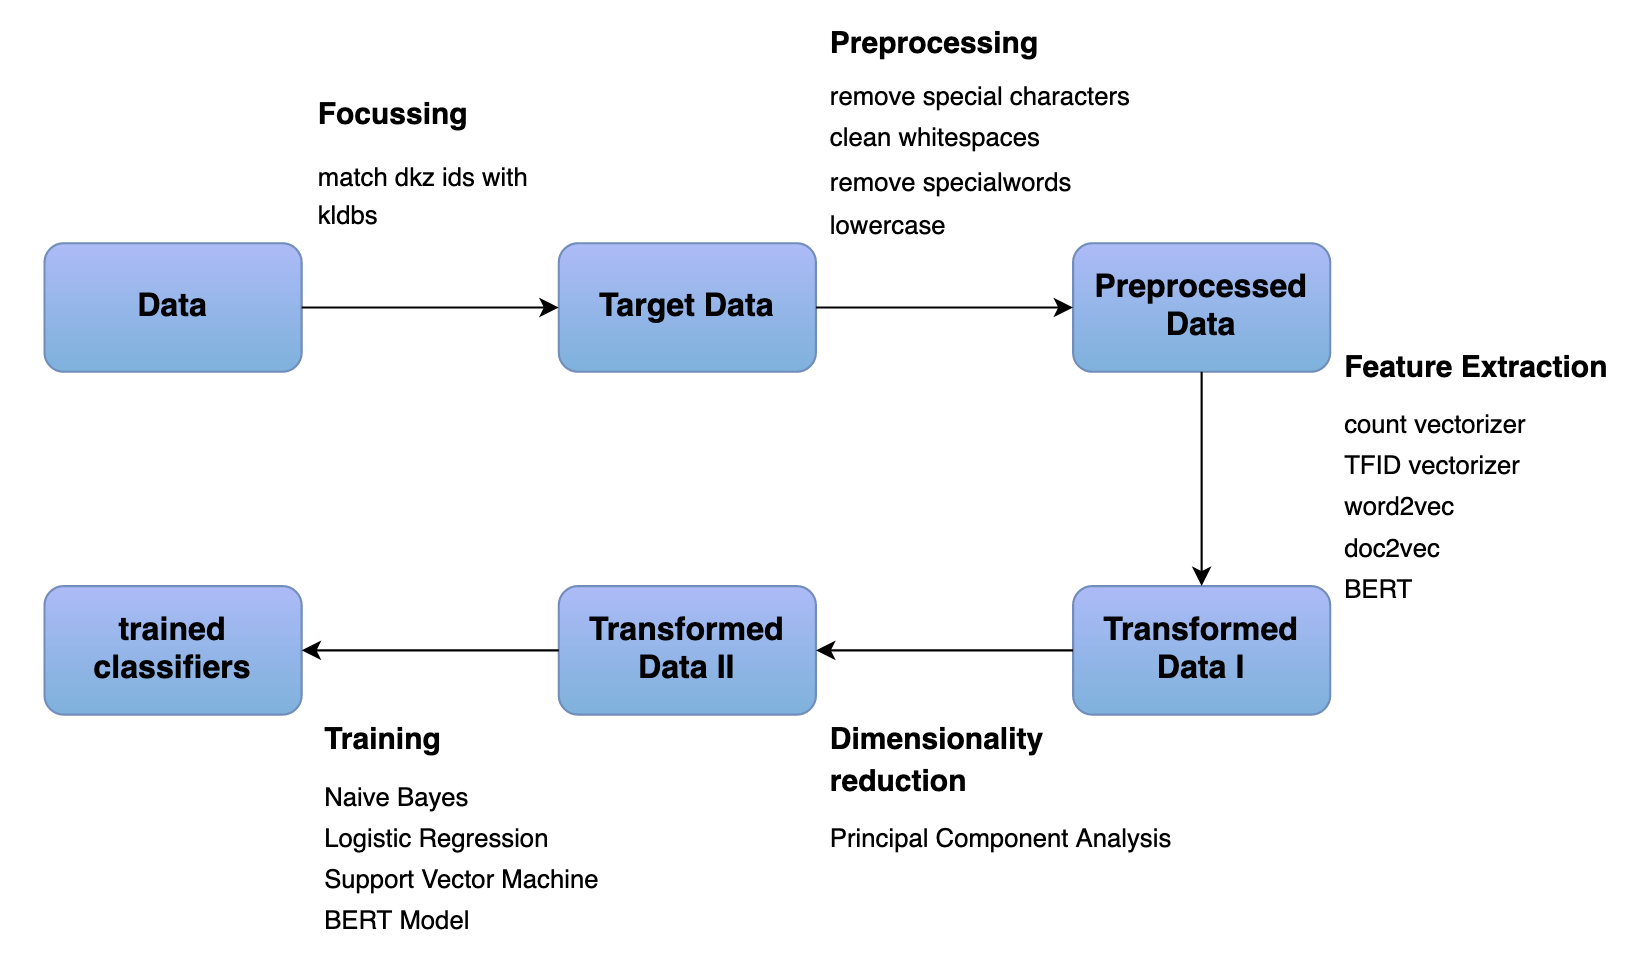
\includegraphics[scale=0.5]{pipeline_MA.png}
  \caption{\label{fig: F8} Training Pipeline}
\end{figure}

The classification process is divided into several steps. Figure \ref{fig: F8} gives an overview of the procedure. In the first step, the \ac{KldB} and the job title data are focused on the necessary variables. This is done by matching the kldb ids from the \ac{KldB} data set with the internal documentation id from the job title data. In the next steps, the targeted data is preprocessed. This preprocessed data is then transformed into numerical vectors. For this purpose, different vector representations are created using five vectorization techniques. The transformed data is then reduced to lower dimensions using principal component analysis. The resulting data is the input for the classifier. In the last step, the four classifiers are trained. Note that the BERT classification algorithm follows a different pipeline, which is why the algorithm is presented separately. Here, the data is used as input to the deep learning model directly after preprocessing and the model is trained. The targeting of the data has already been described in the previous chapter. In the following, the procedure and the associated methods are explained in detail. 

\subsection{Preprocessing}
Preprocessing is crucial step which has to be taken before vectorization. There are several standarized practices for preprocessing like tokenization, stemming, stop-word removal and lowercasing \citep{alsmadi2019}. Preprocessing can have an essential influence on the performance of a classifier \citep{uysal2014, hacohen2020, gonccalves2005}. Therefore, the methods of preprocessing are justified below.

The first preprocessing step is the removal of special characters. This is necessary because most titles contain slashes and brackets to distinguish gender forms in occupational titles. Some job titles contain emojis, such as asterisks, which need to be removed as they are not related directly to specific job titles. 

Capitalized words are usually convert to lowercase in order to treat them equally for the classification. However, lowercase can be at the same time harmful for the performance, if the interpretation changes with converting. Considering the word `US", which refers to the United States of America. Converting to lowercase it is equal to the pronoun `us" and this can affect the performance if the differentiations plays a role for the classification \citep{kowsari2019text}. For occupational names in German, conversion makes sense, since capitalization plays a major role in German. In turn, I don't expect conversion to cause problems often, as described in the example above, since occupational titles usually have their own names and their lowercase variants do not often lead to other words or word classes. Thus in a second step titles are all converted to lowercase. 

As in every text classification task stop words removal is a common praxis. I removed all stopwords, which are listed in the german stopwords list of the Nature Language Toolkit package \citep{bird2009}. In addition to this standardized processes, the data contained other peculiarities that justify further words removal besides stopwords. Job titles very often contain words, such as "employee" or "effective immediately", that do not contain important information and are not specific to particular job titles. These should be removed. To identify a list of such words, the frequencies of each word across all documents are calculated after the aforementioned preprocessing steps. These frequencies are then used to identify words, such as "employee", that are common but not relevant. As a final preprocessing step, the identified words are then also deleted from all job titles. 

\subsection{Vectorization Techniques}
\subsubsection*{Count vectorizer}
The count vectorizer is one of most simple techniques of converting texts to vectors. It belongs to the family of \ac{BOW} models. \ac{BOW} models are based on vectors, where each dimension is a word from a vocabulary or corpus. The corpus is built by all words across all documents. \ac{BOW} models have two important properties. First, they do not consider the order of the words, sequences or the grammar, which is why they also called \ac{BOW}. Second, each word in the corpus is represented by it's own dimension. Thus the vectors contains a lot of zeros, especially for short texts, which is why they belong to the family of sparse vectors \citep{ajose2020}.  Assuming, for example, a corpus contains of 1000 words, meaning each text is built only with these 1000 words, the vector for each text has a length of 1000, thus, producing sparse, high-dimensional vectors \citep{kulkarni2021, sarkar2016}

For the count vectorizer the values for the vector are generated by counting for each text the frequency of the words occuring. Considering a corpus including only the three words ``java", ``developer" and ``python", the titles ``java developer" and ``python developer" would be encoded as follows: 


\begin{table}[hb!]
\center
  \begin{tabular}{llll}
  \hline
                   & java & developer & python \\ \hline
  java developer   & 1    & 1         & 0      \\
  python developer & 0    & 1         & 1      \\ \hline
  \end{tabular}
  \caption{\label{tab: T11} Encoding with count vectorizer}
  \end{table}

The table \ref{tab: T11} results in the vectors $(1,1,0)$ and $(0,1,1)$. Note that if the title ``java developer" contains, for example, two times the word ``java" then the vector would change to (2,1,0). But since this is not a likely case for short text and especially job titles, the count vectorization here is for the most titles similar to one-hot vector encoding, which only considers the occurence of the words, but not the frequency \citep{kulkarni2021, sarkar2016}

While being one of the most simple techniques, count vectorizer has several limitations. The main downside is that it does not consider information like the semantic meaning of a text, the order, sequences or the context. In other words a lot of information of the text is losen \citep{sarkar2016}. In addition, count vectorizer does not take into account the importance of words in terms of a higher weighting of rare words and a lower weighting of frequent words across all documents. \citep{suleymanov2019}

\subsubsection*{TFIDF vectorizer}
\ac{TF-IDF} belongs like the count vectorizer, to the family of \ac{BOW} and is as well a sparse vector. In contrast to count vectorizer, it considers the importance of the words by using the \ac{IDF}. The main idea of \ac{TF-IDF} is to produce high values for words which occur often in a documents, but are rare over all documents. The \ac{TF} represents the frequency of a word t in a document d and is denoted by $tf(t,d)$. The \ac{DF}, denoted by $df$, quantifies the occurence of a word over all documents. By taking the inverse of \ac{DF} we get the \ac{IDF}. Intuitvely the \ac{IDF} should quantify how distinguishable a term is. If a term is frequent over all documents it is not usful for the distinction between documents. Thus the \ac{IDF} produces low values for common words and high values for rare terms and is calculated as follows \citep{sidorov2019, kuang2010}: 

\[idf(t) = log \frac{N}{df} \]

where N is the set of documents. The log is used to attenuate high frequencies. If a term occurs in every document, so $df = N$ the \ac{IDF} takes a value of 0 ($log (\frac{N}{N})$) and if a term is occuring only one time over all documents, thus distinguish perfectly the document from other documents, $idf(t) = log (\frac{N}{1}) = 1$. \citep{sidorov2019} Note that there are slight adjustments to calculate the \ac{IDF}. \citep{robertson2004} The implementation of sklearn package, which is used in this work uses an adapted calculation \citep{scikit-learn}:

\[idf(t) = log \frac{1+n}{1+df(t)} + 1 \] 

Given the $idf(t)$ and $tf$ the \ac{TF-IDF} can be obtained by multiplying both metrics. The implementation of sklearn normalize in addition the resulting \ac{TF-IDF} vectors $v$ by the Euclidean norm \citep{scikit-learn}: 

\[v_{norm} = \frac{v}{||v||_2} \]

Although \ac{TF-IDF} considers the importance of words compared to count vectorizer, as a \ac{BOW} model it suffers from the same limitation as count vectorizer of not taking semantic, grammatic, sequences and context into account \citep{sarkar2016}. 

\subsubsection*{Word2Vec}
In contrast to the sparse techniques method mentioned above, word embedding techniques are another popular approach for vectorization. Word embedding vectors are characterised by low dimensions, dense representation and a continous space. They are usually trained with neural networks \citep{li2015, jin2016}. 

Word2Vec, introduced by \citet{mikolov2013}, is one computionally efficient word embedding implementation. The main idea of Word2Vec is based on the distributional hypothesis, which states that similar words appear often in similar context \citep{sahlgren2008}. Thus, Word2Vec learns with the help of the context representations of words, which includes the semantic meaning and the context. In such a way it words which are similar are encoded similarily \citep{sarkar2016}. 

There exists two variants of Word2Vec. The first variant is based on \ac{BOW}, the so-called \ac{CBOW}, which predicts a word based on surrounding words. In contrast, the second variant, Skip-Gram, predicts the context words from a word \citep{ajose2020, sarkar2016}. Since in this work a pretrained model from Google is used, which is trained with CBOW, in the following the focus is on \ac{CBOW}. 

\ac{CBOW} Word2vec is a 2-layer neural network with a hidden layer and a output softmax layer, which is visualized in figure \ref{fig: F1}. The goal is to predict a word, the so-called target word, by using the target word's context words. The number of context words is defined by a certain window size. If the window size is 2, the 2 words before and the 2 two words after the target word are considered. Given a vocabulary V, which is a the unqiue set of the words from the corpus, each context word c is fed into the neural network, encoded with one-hot encoding of the length of V, building vector $x_c$. Thus in figure \ref*{fig: F1} $x_{1k}$, for example, could be a one-hot encoded vector of the word before the target word. 

\begin{figure}[]
  \center
  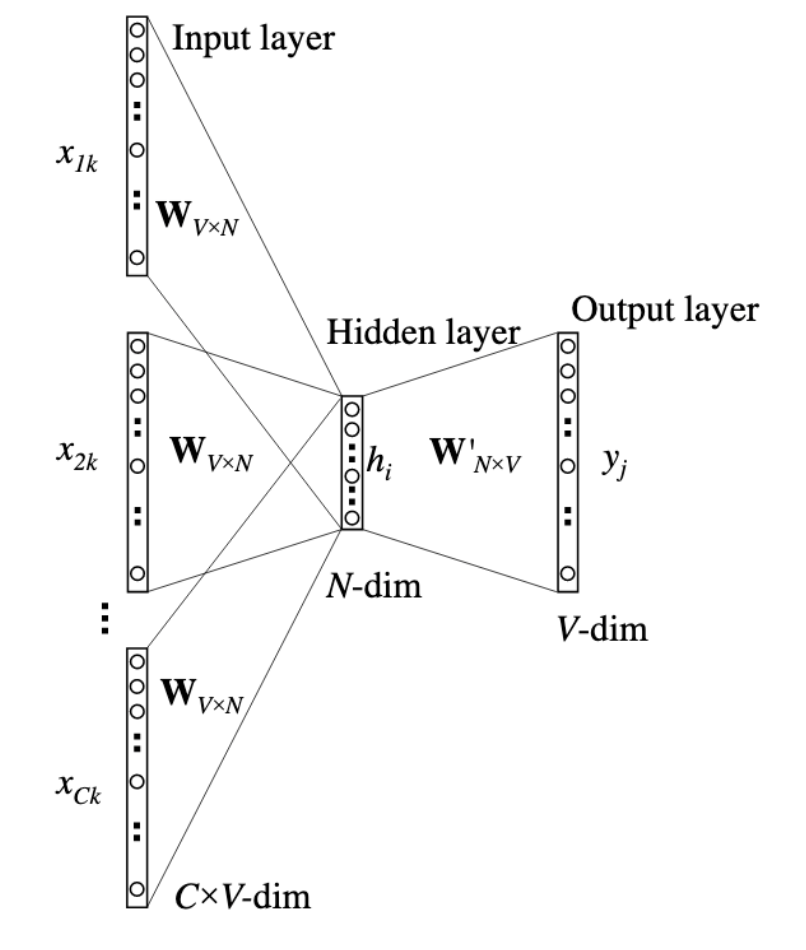
\includegraphics[scale=0.5]{word2vecCBOW.png}
  \caption{\label{fig: F1} \ac{CBOW} \citep[6]{rong2014}}
\end{figure}

The weights between the input layer and the hidden layer are shown in figure \ref{fig: F1}. Taking the dimension of V and N results in the $V \times N$ matrix W. Given that each row $v_w$ in W represents the weights of the associated word from the input and C equals to the number of context words, the hidden layer h is calculated as follows \citep{rong2014}:

\[ h = \frac{1}{C} W^T(x_1 + x_2 + ... +x_c) = \frac{1}{C}(v_{w_1} + v_{w_2} + ... + v_{w_C}) \]

Since the context words are encoded with one hot vector encoding, all except of the respective word value in the vector, which is 1, will be zero. Thus calculating h is just copying the k-th row of matrix W, thus a n-dimensional vector, which explains the second part of the equation. The hidden-layer matrix builds later the word embedding, which is why the decision of the size of the hidden layer defines the dimensions later for the word embedding vector \citep{rong2014}

From the hidden to the output layer a $N \times V$ weight matrix is used to calculate scores for each word in V. A softmax function is used to get the word representation. Caluculating the error and using backpropagation the weights are updated respectivley resulting then in a trained neural network. In practice, due to computional efficiency, instead of the softmax function Word2Vec is trained with hierarchical softmax or negative sampling. Both methods are efficient in the sense that they reduce the amount of weight matrix updates. \footnote{Since the focus is relying here on the word embeddings from the hidden layer and not the trained neural network itself, no further mathematical details will be given concerning the updating. For a detailed derivation see \citep{rong2014}}. \citep{rong2014, simonton2017}. 

Based on the given theoretical insights, I train two Word2vec models. Both models use a pretrained model from Google and are fine tuned with different data. The first model is fine tuned with the complete dataset. The second model includes the additional knowledge. The model setting is as follows: I use \ac{CBOW} Word2Vec models with negative sampling technique. The hidden layer size and thus the word embedding vectors is 300, since the vectors have to have the same size as the pretrained Google vectors, which have a size of 300. The minimal count of words is set to 1. The number of times the training data set is iterated, the epoch number, is set to 10. Lastly, the window size for the context is set to 5. 

As last step the resulting word embeddings need to be processd in some way to get sentence embeddings for each job title. As the name already indicates Word2Vec cannot output sentence embeddings directly. In order to get the sentence embeddings the word vector embeddings of each job title are averaged. 

\subsubsection*{Doc2vec}
Doc2vec, also known as paragraph vectors or Distributed Memory Model of Paragraph Vectors is an extension method of Word2Vec, which outputs directly embeddings for each document \citep{lau2016} It was proposed by \cite{le2014}. Doc2Vec can be used for a variable length of paragraphs, thus it is applicable for bigger documents, but also for short sentences like job titles \citep{le2014}. 

The main idea is, like for Word2Vec, to predict words in a paragraph. To do so, a paragraph vector and word vectors, like in Word2Vec, for that paragraph are concatenated. The paragraph vector `"acts as memory that remembers what is missing from the current contest - or the topic of the paragraph" \citep[3]{le2014}. Therby the paragraph vectors are trained as well with stochastic gradient descent and backpropagation. Similar to Word2Vec practical implementation use hierarchical softmax or negative sampling to fast up training time \citep{lau2016}. 

\begin{figure}[]
  \center
  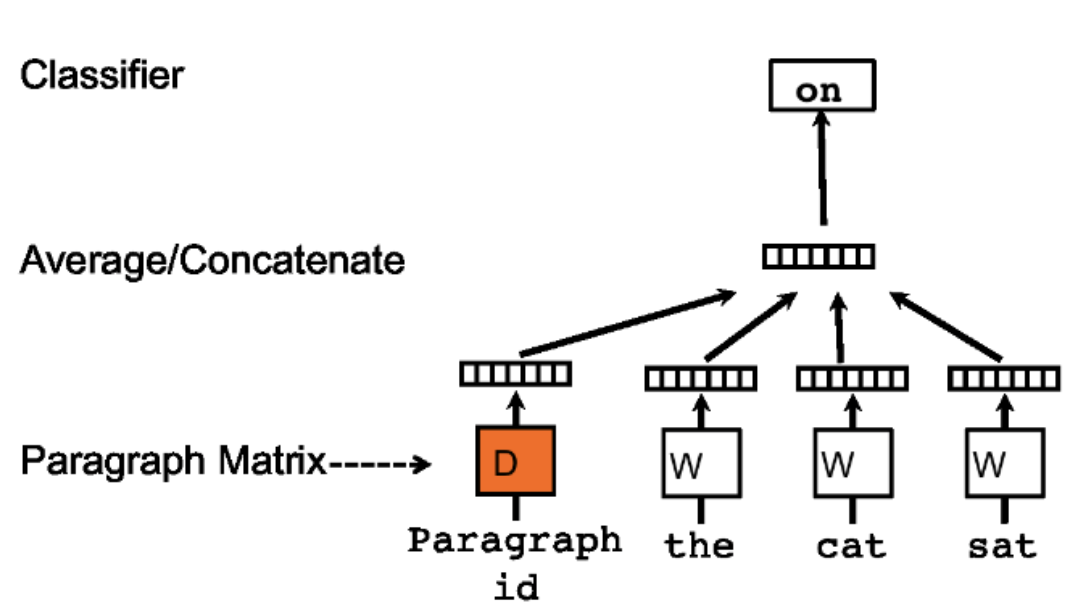
\includegraphics[scale=0.5]{doc2vec.png}
  \caption{\label{fig: F2} Doc2vec - Distributed Memory Model of Paragraph Vectors \citep[3]{le2014}}
\end{figure}

In figure \ref{fig: F2} the algorithm is visualized. As an input the neural networks takes word vectors and a paragraph vector. While the word vectors are shared over all paragraphs, the paragprah vectors are unique for each paragraph. Those paragraphs are represented as unique vectors in a column of a matrix D. The word vectors are respresented in the matrix W as before. In order to predict the word both vectors are combined for example by averaging or concatenating. The Doc2vec implementation described by \citet{le2014} and also used in this work here concatenate the vectors. Formally this only changes the calculation of h. \citep{lau2016}

Since Doc2vec is a word embedding method it has the same advantages mentioned above in the Word2Vec part. In addition Doc2Vec takes the word order into account. At least in the same way of a large n-gram \citep{le2014}. 

Besides the model explained above, Doc2Vec comes also in a second variant, the so-called Distributed Bag of Words of Paragraph model, which ignores the word order. It is not clear which model performs better, although the inventor of Doc2vec propose the first version \citep{lau2016}

Based on this disussion, I created two Distributed Memory Models of Paragraph Vectors. Instead of fine tuning a pretrained model, I trained two custom models, one with the training data and one including the additional knowledge. I set the vector size to 300 with a window size of 5, a minimal count of 1 and trained 10 epochs. Like Word2vec, the models are trained with negative sampling.  

\subsubsection*{BERT}
The last vectorization technique, \ac{BERT}, is the state-of-art language modeling technique developed by \citep{devlin2018} at Google. \ac{BERT} stands out from other langugage models in several ways and outperforms other models for many \ac{NLP} tasks. First, \ac{BERT} uses bidirectional pretraining. Thus is does not only process from left-to-right or right-to-left, but it merge both of them. Second, it is possible to fine tune the model for specific task without heavily-engineered and computionally costly architectures. Third compared to word2vec it is a context-dependent model. Thus, while word2vec would produce only one word embedding for "'Python" \ac{BERT} can give based on the context different embeddings. Here '"Python" as a snake or as a programming language. 

\subsubsection*{Architecture}
\ac{BERT} uses a multi-layer bidirectional Transformer encoder as the architecture. This transformer architecture was introduced by \citet{vaswani2017}. It consists of encoder and a decoder and make use of self-attention. Both, encoder and decoder stack include a number of identical layer, each of them including two sub-layers: a Multi-head attention and a feedforward network layer \footnote{A simplified visualization with a two layer encoder, as well the architecture of a  can be found in the Appendix.} It is out of the scope to elaborate the technical details and implementation of the attention mechanism, which is why in the following a simplified explanation of the attention mechanism is given. 

The self-attention mechanism improves the representation of a word, represented by a matrix X, by relating it to all other words in the sentence. In the sentence '"A dog ate the food because it was hungry"' \citep[10]{ravichandiran2021} the self-attention mechanism, for example, could identify by relating the word to all other words, that '"it" belongs to '"dog" and not to '"food". 
In order to compute the self attention of a word three additional matrices, the query matrix Q, the key matrix K and a value matrix V are introduced. Those matrices are created by introducing weights for each of them and multiplying those weights with X. Based on those matrices, the dot product between the Q and the K matrix, a normalization and a softmax function are applied in order to calculate an attention matrix Z  \footnote{For a step-by-step calculating see \citep{ravichandiran2021}}. \ac{BERT} uses a multi-head-attention, which simply means that multiple Z attention matrices instead of a single one are used.

\ac{BERT} takes one sentence or a pair of sentences as input. To do so it uses WordPiece tokenizer and three special embedding layers, the token, the segement and the position embedding layer for each token, which is visualized in \ref{fig: F4}. A WordPiece tokenizes each word which exits in the vocabulary. If a word does not exists words are splitas long a subword matches the vocabulary or a individual character is reached. Subwords are indicated by hashes. For the token embeddings the sentence is tokenized first, then a [CLS] is added at the beginning of the sentence and [SEP] token at the end. For example the job title `"java developer" and `" python developer"' becomes to tokens as shown in the second row of \ref{fig: F4}. In order to distinguish between the two titles a segment embedding is added, indicating the sentences. Last the \ac{BERT} model takes a position embedding layer, which indicates the order of the words. For each token those layers are summed up to get the representation for each token \citep{devlin2018,ravichandiran2021}.

\begin{figure}[hb!]
  \center
  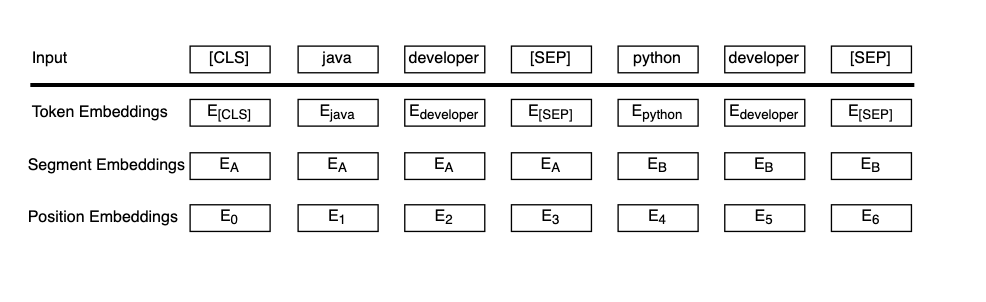
\includegraphics[scale=0.5]{BERTInput_own.png}
  \caption{\label{fig: F4} Input \ac{BERT} \citep[5]{devlin2018}}
\end{figure}

\begin{figure}[hb!]
  \center
  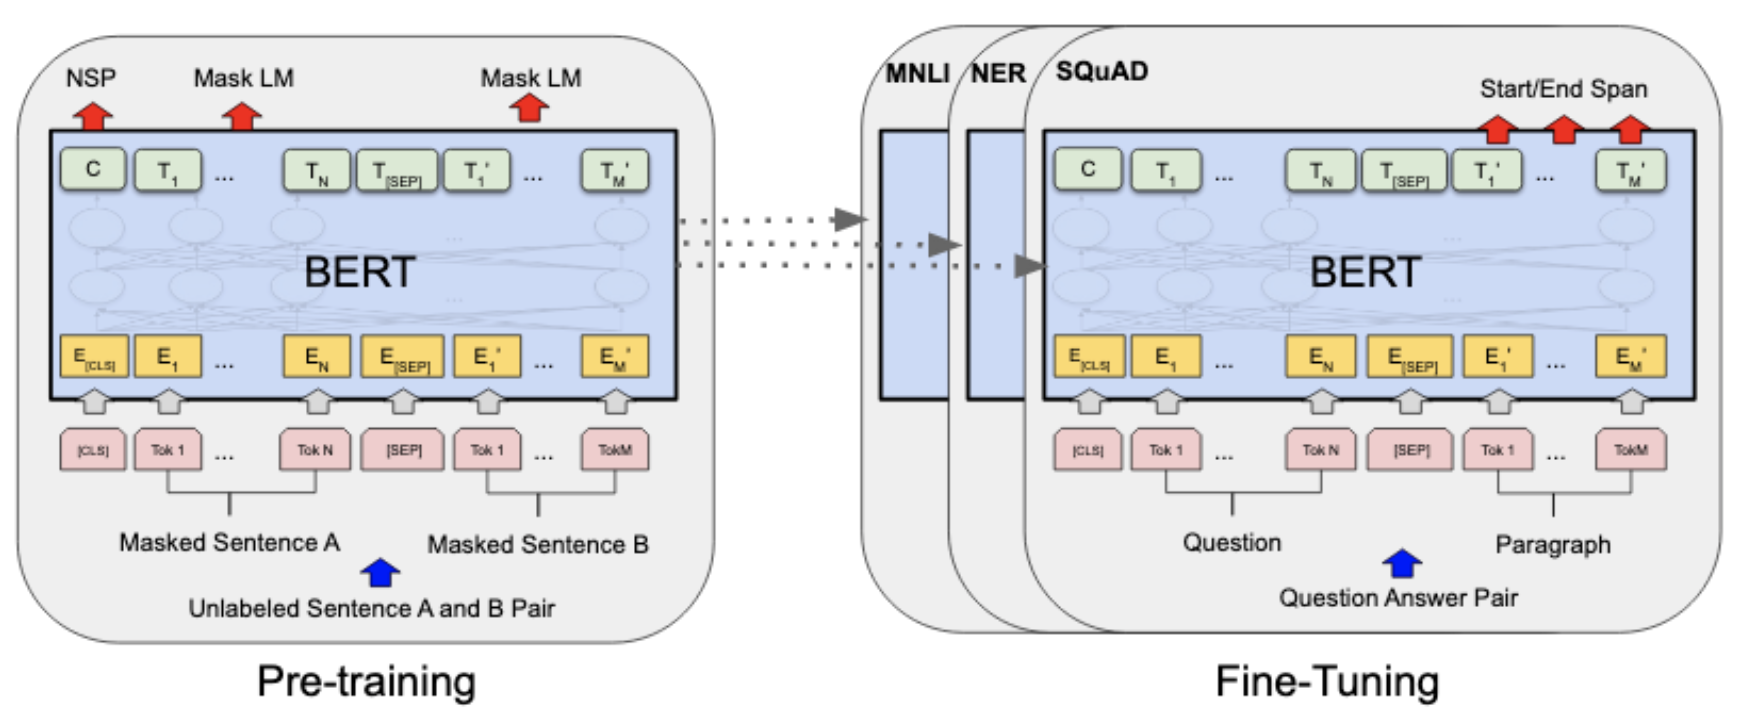
\includegraphics[scale=0.5]{BERTOverview.png}
  \caption{\label{fig: F3} Overview \ac{BERT} \citep[3]{devlin2018}}
\end{figure}


The \ac{BERT} algorithm can be described in two steps. First the pretraining phase, which is illustrated on the left-hand side of the figure \ref{fig: F3} and the fine-tuning phase, visualized on the right-hand side of figure \ref{fig: F3}. The pretraining phase consists of two jobs: Masked language modeling and next sentence prediction. 

\subsubsection*{Pretraining}
Masked language modeling means that a percentage of the input tokens are masked at random. For example the job title `"python developer" could be masked as follows: [[CLS] python [MASK] [SEP]]. Since in fine tuning tokens are not masked a mismatch would occur between fine tuning and pretraining, which is why not all of the masked tokens are actually matched with a [mask] token, but also with random token or the real tokens \footnote{There are specific rules of how to mask. See \citet{devlin2018} for detailed implementation}. Instead of predicting the complete sentence, BERT trains to predict the masked tokens. The prediction is performed with a feed forward network and a softmax activation \citep{devlin2018,ravichandiran2021}. 

The second task takes again two sentences, but predict whether the second sentence follows the first one. This helps to understand the relationship between the sentences. Each sentence pair is labelled with either isNext or NotNext. By using the [CLS] token, which has the aggregating representation of all tokens, a classification task of whether a sentence pair is isNext or NotNext can be carried out \citep{ravichandiran2021,devlin2018}

The pretraining of \ac{BERT} is in contrast to the fine tuning process computionally expensive. Therefore, \citet{devlin2018} initially developed different sizes of \ac{BERT} like \ac{BERT}-base and \ac{BERT}-large. Besides those two models, there are plenty of pretrained \ac{BERT} models for the German case, like \ac{BERT}-base-german-cased or distilbert-base-german-cased \footnote{All german \ac{BERT} are open source and are accessible through the transformers library \citep{wolf2020}}. In an evaluation of German pre-trained language models, \citep{assenmacher2021} conclude that the bert-base-german-dbmd-uncased algorithm works quite well. Following their results and own tests on different mode bert-base-german-dbmd-uncased seems to have the best result, which is why I use it for the fine tuning process. The model consists of 12 encoder layers, denoted by L, 12 attention heads, denoted by A and 768 hidden units, which results in total in 110 million parameters. It was trained with 16GB of German texts. 

\subsubsection*{Fine-Tuning}
The second phase, the fine-tuning, can be performed in different ways, also depending on the task. For text classifcation there are two main strategies. Either the weights of the pretraind model are updated during the classifcation process. Or the pretrained model is first fine-tuned and then used as a feature extractor.  Such it can be then in turn used for, for example, calculating similarities or as an input for classification algorithms. 

I train two models with \ac{BERT}. While the first model includes a classifcation layer, in the following named as \ac{BERT} classifier, the second model applies \ac{BERT} as a feature extraction method, in the following named \ac{BERT} vectorizer. 

The \ac{BERT} classifier is fine tuned with the complete training data set. Practically this is done by converting the sentences of the dataset to the appropriate data format as described above and train it with the supervised dataset on some epochs, which then outputs  the labels. From a theoretical point of view the last hidden state of the [CLS] token with the aggregation of the whole sentence is used for the classifcation. In order to get the labels \ac{BERT} uses a softmax function \footnote{The explanation of the softmax function follows in the chapter of the classifiers} \citep{sun2019}. As already state in the literature review in the literature it is not well-understood so far, what exactly happens during the fine-tuning. An analysis of \citet{merchant2020} indicates that the fine tuning process is relatively conservative in the sense that they affect only few layers and are specific for examples of a domain. Note that this analysis focussed on other nature language processing task than text classifcation. The set-up of the training is as follows: Testing different epoch numbers indicates that lower epoch size have better results for the model, which is why I fine tune in 6 epochs. For the optimization an adam algorithm, a gradient based optimizer \citep{kingma2014}, with a learning rate of $1e^{-5}$ is used. 

In order to get sentence embeddings different strategies, like averaging the output layer of \ac{BERT} or using the [CLS] token, are applied. Another method, developed by \citet{reimers2019} is Sentence-\ac{BERT}, which is computionally efficient and practicable to implement. Thus, it faciliate to encode sentences directly into embeddings, which is why I use it for the \ac{BERT} vectorizer. The model is constructed with the bert-base-german-case model and a pooling layer. The pooling layer is added to output the sentence embeddings. The fine tuning process uses a siamese network architecture to update the weights. \ref{fig: F5} shows the architecture. The network takes pairs of sentences with a score as an input. Those scores indicate the similarity between the sentences. The network update the weights by passing the sentences through the network, calculating the cosine similarity and comparing to the similarity score \citep{reimers2019}.
I create from the job title dataset and from the kldb dataset pairs of similar and dissimilar job titles or searchwords. Similar pairs are pairs from the same kldb class. As a score I choose 0.8. Dissimilar pairs are defined as pairs which are not from the same class. The score is 0.2. Building all combinations of titles and the searchwords for each class would results in a huge dataset. For example class 1 of the training data set has 2755 job titles. Thus we would have already have ${2755 \choose 2} = 3793635$ examples. Since this is computionally too expensive I randomly choose pairs of job titles. For level 1 the following samples are drawn: From the job title data for each class I used 3250 pairs. The same also for the searchwords for each class. For unsimilar pairs I used 1750 job titles pairs which are not from the same class. Same for searchwords. This results in total number of $(3250+3250) \times 9 + 2 \times 1750 = 62000$ pairs for the finetuning of level 1. \footnote{The determination of the exact number of pairs is exploratory in character, and run time and performance were taken into account}. For level 3 the procedure is the same, only the numbers differs. I used for similar pairs for job titles and searchwords 400 for each class and for the unsimilar 6000 pairs, which gives a total number of $(400 + 400) \times (136-7) + 2 \times 1500 =  61200$. Classes with only one example are not considered, because building pairs is not possible. 

\begin{figure}[hb!]
  \center
  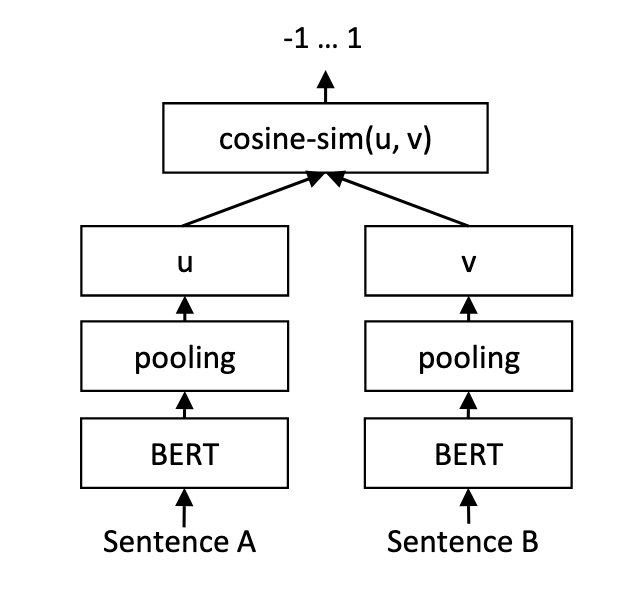
\includegraphics[scale=0.5]{SBERT.png}
  \caption{\label{fig: F5} Sentence-\ac{BERT} siamese architecture \citep[3]{reimers2019}}
\end{figure}

\subsection{Dimensionality reduction}
Dimensionality reduction techniques like \ac{PCA} play an important role in reducing computation time and saving computing resources \citep{ayesha2020}. Figure \ref{fig: F6} shows the running time of all three classifiers with different data sizes and with and without \ac{PCA} dimensionality reducation. 


\begin{figure}[hb!]
  \center
  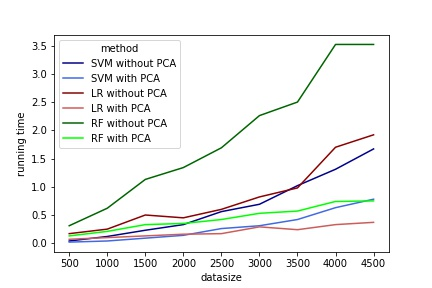
\includegraphics[scale=0.5]{running_time_PCA.jpeg}
  \caption{\label{fig: F6} Running time of word2vec with different data sizes}
\end{figure}

The input of the classifiers are the word2vec word embeddings without the additional information. The bright lines show the running times without dimensionality reduction, while the dark colored lines report the running time with \ac{PCA} transformation. It becomes clear that the runtime for the transformed embeddings are generally lower. While the magnitude of the differences is almost irrelevant for a data set of 500, the runtime of the non-transformed embeddings increases considerably with the size of the data set for all classifiers. This is most evident with \ac{RF}. Although the runtime of the transformed embeddings also increases for all classifiers, it does so at a much slower pace. Therefore, it can be concluded that the transformation clearly contributes to keeping the runtime lower for large data sets. As already described in chapter x, the training data set is fairly large, which is why it is reasonable to reduce the dimensions. 

\ac{PCA}, one of the most popular technique for dimensionality reduction, aims to reduce a high-dimensional feature space to a lower subspace while capturing the most important information \citep{tipping1999, bisong2019}. The main idea is to use linear combinations of the original dimensions, so called principal components, to reduce the dimensional space \citep{bro2014,geladi2017}. 

Conceptually in the first step the covariance matrix for the word embeddings, is obtained. The covariance matrix, denoted by $\textbf{X}$, captures the linear relationships between the features of the word embeddings. In a next step the eigenvectors of $\textbf{X}$ are calculated. The eigenvector of X defined as \citep{bro2014}: 

\[ \textbf{X}z = \lambda z \]

where $z$ is the eigenvector and $\lambda$ the eigenvalue. In order decompose $\textbf{X}$ to get the eigenvalue Singular Value Decomposition is applied. The eigenvalues are then sorted from highest to lowest and the most significant components n are kept. To transform the data a feature vector in generated. This vector contains of the most n significant eigenvalues. After transposing the mean-adjusted the word embedding and the feature vector, the embeddings can be transformed by multiplying both transposed vectors \citep{smith2002}.

\subsection{Classifier}
As pointed out in the literature review \ac{NB}, \ac{MLR} and \ac{SVM} have several advantages for text classifcation tasks. In the following based on a theoretical discussion of each classifier, the exact modeling of the classifiers is justified. The focus and the depth of the explanations of the classifier's characteristics like optimization and decision function, loss or regularization depends on the complexity and the need of explanation in order to understand the basic principle of the classifiers and thus are not all equally structured. 

\subsubsection{Logistic Regression}
\ac{MLR}, a generalized linear model, is one of the most used analytical tools in social and natural science for exploring the relationships between features and categorical outcomes. For solving classification problems it learns weights and a bias(intercept) from the input vector. Figure \ref{fig: F7} illustrate the idea of the calculation of \ac{MLR}. To classify examples first the weighted sum of the input vector is calculated. For multiclassfication the weighted sum has to be calculated for each class. Thus given a $f \times 1]$ feature vector x with $[x_1, x_2, ..., x_f]$, a weight vector $w_k$ with $k$ indicating the class k of set of classes K, a bias vector $b_k$ the weighted sum the dot product of $w_k$ and $\textbf{x}$ plus the $b_k$ defines the weighted sum. Representing the weight vectors of each class in a $[K \times f]$ matrix $\textbf{W}$, formally the weighted sum is $\textbf{W}x+b$. In Figure \ref{fig: F7} the blue lines for example are a row in $\textbf{W}$ and are the weight vectors related to a class labelled with 1 \citep{jurafsky2021}.

\begin{figure}[hb!]
  \center
  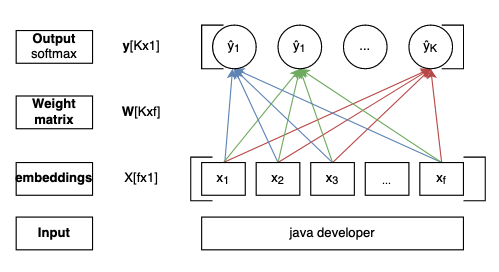
\includegraphics[scale=0.5]{LR.png}
  \caption{\label{fig: F7} Multinomial Logistic Regression (edit after \citep[p.]{jurafsky2021})}
\end{figure}

In a second step the weighted sums are mapped to a value range of $[0,1]$ in order to actually classify the input. While binary logistic regression uses a sigmoid function to do so, for \ac{MLR} needs a generalized sigmoid function. This generalization is called the softmax function which outputs probabilities for each of the classes, which is why \ac{MLR} is also often called softmax regression in the literature. These probabilties models for each class $p(y_k = 1|x)$.

Similar to sigmoid function, but for multiple values the softmax function maps each value of an input vector z with $[z_1, z_2, ..., z_K]$ to a value of the range of $[0,1]$. Thus outputting a vector of length z. All values together summing up to 1. Formally it is defined as: 
\[ softmax(z_i) = \frac{exp(z_i)}{\sum^K_{j=1} exp(z_j)} \text{ } 1 \leq i \leq K \]
Then the output vector y can be calculated by 

\[ \hat{y} = softmax(\textbf{W}x+b) \]

Considering the training of the weights and the bias the goal is to `"maximize the log probability of the true y labels" of the input data. This is commonly done by minimizing a generalized cross-entropy-loss function for \ac{MLR}. There exists different methods for solving the optimization problem, like stochastic gradient descent or limited-memory Broyden-Fletcher-Goldfarb Shannon solver. The latter converges rapidly and is characterized by a moderate memory, which is why it can converges faster for high-dimensional data \citep{fei2014, scikit-learn}. 

For \ac{MLR} it is common to add regularization parameter. This avoids overfitting and ensures that the model is more generalizable to unseen data. The idea is to penalize weights which have a good classifaction, but use a lot of high weights, more than weights with good classification but smaller weights. There are two popular penality term, the L1 and the L2 penalty. 
While for L1 the absolute values of the weights are summed and used as the penality term, L2 regualizes \textcolor{red}{with a quadractic function of the weights}. With the regularization a parameter C is introduced to control the strength of the regularization, with C being a positive value and smaller C regulizing stronger. 

The following setting will be used for the \ac{MLR}: A \ac{MLR} with L2 penality with a C value of 1 is used. Since the input vectors, especially for count vectorizer and for \ac{TF-IDF} are high-dimensional the limited-memory Broyden-Fletcher-Goldfarb-Shannon solver is set for solving. For some trainings converge problems appeared, which is why the maximal iteration of the classifier is set to 10000.

\subsubsection{Support Vector Machines}
However, \ac{SVM} also performed well for text classification. Especially for multiclass tasks, as mentioned in the literature review, often different versions of the algorithm are used and showed good performance \citep{Aiolli2005,Angulo2003,Benabdeslem2006,Guo2015,Mayoraz1999,Tang2019,Tomar2015}. In general \ac{SVM} has several advantages for text classifcation. First, text classifcation usually has a high dimensional input space. \ac{SVM} can handle these large features since they are able to learn independently of the dimensionality of the feature space. In addition \ac{SVM}s are known to perform well for dense and sparse vectors, which is usually the case for text classification \citep{Joachims1998}. Empirical results, for example \citet{Joachims1998} or \cite{Liu2010} confirm the theoretical expectations. It is, therefore, a reasonable option to use a basic version of the \ac{SVM} algorithm as a baseline. 

The general idea of a \ac{SVM} is to map ``the input vectors x into a high-dimensional feature space Z through some nonlinear mapping chosen a priori [...], where an optimal separating hyperplane is constructed'' \citep[138]{Vapnik2000}. In \ac{SVM} this optimal hyperplane maximizes the margin, which is simply put the distance from the hyperplane to the closest points, so called Support Vectors, across both classes \citep{Han2012}. Formally, given a training data set with n training vectors $x_i \in R^n, i = 1,....,n$ and the target classes $y_1,...y_i$ with $y_i \in \{-1, 1\}$, the following quadratic programming problem (primal) has to be solved in order to find the optimal hyperplane:
\[\min_{w,b} \frac{1}{2}w^{T}w \] 
\[\text{subject to } y_i(w^T\phi(x_i)+b) \geq 1\]

where $\phi(x_i)$ transforms $x_i$ into a higher dimensional space, $w$ corresponds to the weight and $b$ is the bias \citep{Chang2001,Jordan2006}
The given optimzation function assumes that the data can be separated without errors. This is not always possible, which is why \cite{Cortes1995} introduce a soft margin \ac{SVM}, which allows for missclassfication \citep{Vapnik2000}.
By adding a regularization parameter $C$ with $C > 0$ and the corresponding slack-variable $\xi$ the optimization problem changes to \citep{Chang2001, Han2012}: 
\[\min_{w,b} \frac{1}{2}w^{T}w + C \sum_{i=1}^n \xi_i \] 
\[\text{subject to } y_i(w^T\phi(x_i)+b) \geq 1 - \xi_i, \] 
\[\xi_i \geq, i = 1,...,n\]

Introducing Lagrange multipliers $\alpha_i$ and converting the above optimization problem into a dual problem the optimal $w$ meets \citep{Chang2001, Jordan2006}:
\[w = \sum_{I=1}^n y_i\alpha_i\phi(x_i)\]

with the decision function \citep{Chang2001}:
\[\text{sgn } (w^T\phi(x)+b) = sgn(\sum_{i=1}^n y_i \alpha K(x_i, x) +b)\]

$K(x_i, x)$ corresponds to a Kernel function, which allows to calculate the dot product in the original input space without knowing the exact mapping into the higher space \citep{Han2012, Jordan2006}. 

In order to apply \ac{SVM} to multiclass problems several approaches have been proposed. One stratetgy is to divide the multi-classifcation problem into several binary problems. A common approach here is the one-against-all method. In this method as many \ac{SVM} classifiers are constructed as there are classes k. The k-th classifier assumes that the examples with the k label are positive labels, while all the other examples treated as negative. Another popular approach is the one-against-one method. In this approach $k(k-1)/2$ classifiers are constructed allowing to train in each classifier the data of two classes \citep{Hsu2002}. Besides dividing the multiclass problem into several binary problems, some researches propose approaches to solve the task in one single optimization problem, like \citet{Crammer2001}. \footnote{For a detailed overview of all different methods and the method of \citet{Crammer2001} see \citet{Hsu2002,Crammer2001}}. 

In order to find a strong classifier I checked \ac{SVM}'s with different parameters for the \ac{SVM}, as well as different multiclass approaches. It appears that a SVM using a soft margin with a $C=1$ and a one-vs-rest approach has the best results. I also test different kernels, like  RBF Kernel or linear kernel. The linear kernel, formally  $k(x, x') = x^Tx'$, achieved the best results, which is why I choose it for the classifier. 


\subsubsection{Random Forest Classifier}
In contrast to the previous two classifiers \ac{RF} is a ensemble learning technique. The main idea of ensemble learning techniques is to create a number of learners, classifiers, and combine them. Those learners are for example descision tree or neural networks and are usually homogeneous, which means that each individual learner is based on the same machine learning algorithm. The different ensemble techniques are built on three pillars: the data sampling technique, the strategy of the training and the combination method \cite{polikar2012, zhou2009}. 

The first pillar, the data sampling is important in sense of that it is not desirable to have same outputs for all classifiers. Thus ensemble techniques need diversity in the output, which means the outputs should be optimally independent and negatively correlated. There are well-established methods for achieving diversity. For example bagging techniques \ac{RF} falls back to boostrap \citep{polikar2012}. The second pillar rises the question of which techniques should be applied to train the learners of the method. The most popular strategies for the training are bagging and boosting \citep{polikar2012}. The last pillar is about the combining method. Each classifier of the method will output an individual classifcation result and those results have to be combined in some way to achieve an overall result. There are plenty of methods like majority voting or borda count \citep{polikar2012}.

\ac{RF} uses as individual classfier decision trees. Before discussing \ac{RF} in more detail within the three pillars described above, a brief discussion of decision tree is given, in order to understand the mechanism and training procedure of the classifiers. 

The main idea of the decision tree algorithm is to `"break up a complex decision into a union of several simple decisions" \citep[660]{safavian1991} by using trees, with a root node on the top, intermediate nodes and leaf nodes on the bottom. For the root node and each of the intermediate nodes all possible splittings are checked and then are split according to the best feature. Each leaf nodes leads to one of the classification labels. Examples are then classified by traversing the tree from the top to the bottom and choosing at each intermediate node the branch which satisfy the attribute value for the example. The construction of a Decision tree is a recursive procedure \citep{Berthold2020, xia2008, cutler2012}. The algorithm stops for a specific node if all examples of the training set belong to the same class, or if there are no features left for splitting. This might end in tree with a high depth, which is why often pruning is applied to avoid overfitting of the tree \citet{Berthold2020}.

There are two important points to discuss in constructing. First the types of splitting and second splitting criterion. There are mainly three types of splits: Boolean splits, nominal splits and continous splits. The latter chooses a particular value from the continous feature as the splitting value \citep{cutler2012, Berthold2020}. For example considering a word embedding x with 300 dimension and a node t of a decision tree, which is split into a nodes $t_{left}$ and $t_{right}$. The node t could have the split $x[209] <= 0.336$. Examples with a value smaller than or equal $0.336$ at the dimension index $209$ of the embedding vector are follow the branch to $t_{left}$, while all other examples follow the branch to $t_{right}$.

The splitting criterion is important to identify the best feature for splitting. Intiutively, the criterions should split the data in such a way that leaf nodes are created fast \citep{Berthold2020}. There are several measurements, so-called impurity measures to obtain the best split for each node, like gini impurity or information gain. Since \ac{RF} uses gini impurity, only this criterion will be discussed in detail. 

The gini value indicates the purity of a dataset D with n classes. It is defined as follows \citep[3156]{yuan2021}: 

\[Gini(D) = 1 - \sum_{i=1}^n p^2_i\]

$p_i$ is th probability that a class n occurs in D. The more pure D is the lower the value of the gini value. To determine the best feature k, the dataset is partitioned based on the feature k. For continous features, as in word embeddings, this is done by continous split. Defining V as the total number of subsets and $D^v$ as one of the subsets, the gini impurity for a feature k can be calculated as follows \cite{yuan2021}: 

\[\text{Gini index}(D,k) = \sum_{v=1}^V \frac{|D^v|}{|D|} Gini(D^v) \]

Conceptually the Gini index is the weighted average of the gini value for each subset of D based on a feature k. Thus subsets with more samples are weighted more in the gini index. The optimal feature $k^*$ is then determined by minimizing the Gini impurity over all features K \citep[3156]{yuan2021}: 

\[ k^* = arg \min_{k \in K} \text{Gini index} (D,k) \]. 

Based on above theoretical explanations of the foundations of decision tree, researchers have developed several algorithms to train decision trees, like Iterative Dichotomiser 3, C4.5. or \ac{CART}, which is used in \ac{RF}. \ac{CART} produces depending on the target variable classification (for categorical variables) or regression trees (for numerical variables). It constructs only binary trees, thus each split is into two nodes. The algorithm uses as impurity measurement gini index and it can handle numerical and categorical input \citep{brijain2014}.

\ac{RF} belongs to the family of bagging ensemble techniques.
Bagging selects a single algorithm and train a number of independent classifiers. The sampling technique is sampling with replacement (bootstrapping). Bagging combines the individual models by using either majority voting or averaging. \ac{RF} differentiates from the classic bagging method in the way that it also allows to choose a subset of features for each classifier from which the classifiers can select instead of  allowing them to select from the complete range of features \citep{polikar2012, zhou2009, Berthold2020}. 

Formally \citet{breiman2001}, who introduced mainly the \ac{RF} algorithm defines the classifier as follows:

\begin{quote}
`"A random forest is a classifier consisting of a collection of tree-structured classifiers $\{h(\textbf{x}, \Theta_k), k = 1, ...\}$ where the ${\Theta_k}$ are independent identically distributed random vectors and each tree casts a unit vote for the most popular class at the input $\textbf{x}$." \citep[6]{breiman2001}. 
\end{quote}
$\Theta_k$ is a random vector which is created for each k-th tree. It is important, that $\Theta_k$ is independent of the vectors $\Theta_1...\Theta_{k-1}$, thus from all random vectors of the previous classifiers. Although the distribution of the random vectors remain. Combined with the training set, with $\textbf{x}$ as the input vector a classifier $h(\textbf{x}, \Theta_k)$ is constructed \citep{breiman2001}. In practical implementation the random component $\Theta_k$ is not explicitly used. Instead it is rather used implicitly to generate two random strategies \citep{cutler2012}. The first strategy is the bootstrapping. Thus drawing sample with replacement from the training data set. In order to estimating generalization error, correlation and variable importance \citet{breiman2001} applied out-of-bag estimation. Out-of-bag estimation leave out some portion of the training data in each bootstrap. The second strategy is to choose random feature for the splitting. Thus at each node from the set of features only a subset is used to split. While decision trees are often pruned to avoid overfitting, \ac{RF} does without. The trees grow by applying \ac{CART}-algorithm. \ac{RF} uses as combination method for classifcation unweighted voting \citep{cutler2012}.

Based on the above explanations the implemented \ac{RF} has the following setting: The numbers of learners is 100. Gini is used as the splitting criterion. The maximal number of features is $\sqrt{\text{number of features}}$. Note that sklearn, which is used to implement \ac{RF} here, uses an optimised algorithm of \ac{CART}. \citep{scikit-learn}.

 

\section{Result}
\subsection{Evaluation metrics}
There exists several metrics for the evaluation of classification approaches in the literature \citep{Fatourechi2008}. The choice of appropriate measurements is a crucial step for obtaining a qualitative comparison in the performance between the baseline algorithms and the new approaches. Often researchers rely on popular metrics like \ac{OA}. However, especially for multiclass and inbalanced dataset tasks it is difficult to rely only on one measure like \ac{OA} In order to select appropriate metrics for comparison in the following the most important metrics will be discussed focussing on multiclass classification and imbalanced data sets. 

Most metrics rely on a confusion matrix. For the multiclass case this confusion matrix is defined as follows \citep{Kautz2017}: 
\begin{table}[hb!]
  \center
  \begin{tabular}{lllll}
  \hline
            & positive examples      &           &             &             \\ \hline
  positive prediction  & $c_{1,1}$ & $c_{1,2}$ & $\dots$     & $c_{1,n}$   \\
            & $c_{2,1}$ & $c_{i,j}$ &             &             \\
            &  $\vdots$         &           & $\ddots$ &   $\vdots$\\
            & $c_{n,1}$ &           & $\dots$     & $c_{n,n}$   \\ \hline
  \end{tabular}
  \caption{\label{tab: T1} Confusion Matrix (edited after \citep[113]{Kautz2017}}
  \end{table}

From the confusion matrix follows that $c_{i, j}$ defines examples which belong to class j and are predicted as class i. Given that $k$ is the current class, \ac{TP} is defined as $tp_{k} = c_{k, k}$, thus examples which are correctly predicted as the current class k. \ac{FN} are defined as those examples which not belonging to the current class k, but are predicted as k. Formally $fn_{k} = \sum_{i=1, i \neq k}^n c_{i, k}$. Next, \ac{TN}, are examples belonging to the current class m, but are not predicted as m. Formally $tn_{k} = \sum_{i=1, i\neq k}^n \sum_{j=1, j \neq k}^n c_{i,j}$. Last, \ac{FP} are defined as examples not belonging to class k, but are predicted as such. Formally this can be expressed as: $fp_{k} =  \sum_{i=1, i \neq k}^n c_{k, i}$ \citep{Kautz2017}

As mentioned the \ac{OA} is one of most common metric for performance evaluation. It represents how well the classifier classifies across all classes correctly. Formally, given that N is number of examples and K the number of all classes, this can be expressed as \citep{Branco2017}: 
\[OA = \frac{1}{K} \sum_{i = 1}^K \frac{tp_{k} + tn_{k}}{N}\]
% \[OA = \frac{TP+ TN}{n}\]
Following the formula an accuracy of 1 means that all examples are correctly classified, while a 0 mean that each example is classified with the wrong class. \citep{Berthold2020}
Although \ac{OA} is a widley used metric it is critized for favouring the majority classes, thus not reflecting minority classes appropriatly in unbalanced datasets \citep{Berthold2020, Fatourechi2008}

Two more popular metrics are precision and recall. Precision respresents how well the classifier detects actual positive examples among the positive predicted examples. Recall, also called sensitivity, in contrast, represents how many examples are labelled as positive among the actual positive examples \citep{Berthold2020}. For the multiclass scenario, two different calculation approaches for each of the metrics are proposed: micro and macro average \citep{Branco2017}. In the macro approach first the metric is calculated for each class k against all other classes. The average of all of them is built. Formally: 

\[precision_{macro} = \frac{1}{K} \sum_{i=1}^k \frac{tp_{i}}{tp_{i} + fp_{i}}\]
\[recall_{macro} = \frac{1}{K} \sum_{i=1}^k \frac{tp_{i}}{tp_{i} + fn_{i}}\]

In contrast the micro approach aggregates the values, which can be formally expressed as follows: 

\[precision_{micro} = \frac{\sum_{i=1}^K tp_i}{\sum_{i=1}^K tp_i + fp_i}\]
\[recall_{micro} = \frac{\sum_{i=1}^K tp_i}{\sum_{i=1}^K tp_i + fn_i}\]

There is a trade-off between precision and recall \citep{Buckland1994}. The F-measure capture both precision and recall by taking the harmonic mean between both. It is calculated as follows \citep{Branco2017,Pan2016}:  

\[F_{micro} = 2 \cdot \frac{precision_{micro} \cdot recall_{micro} }{precision_{micro} + recall_{micro} }\ \]

\[F_{macro} = 2 \cdot \frac{precision_{macro} \cdot recall_{macro} }{precision_{macro} + recall_{macro} }\ \]

Apart from the trade-off between recall and precision, there is also a tradeoff between sensitivity and specificty (1- sensitivity). Using a \ac{ROC}, which plots the specifity against the sensitivity the trade-off can be visualized for different thresholds. The area under the curve then can be used to obtain the performance of the classifier. A large area indicates a better classifier \citep{Berthold2020, Espindola2005}. 

As shown above, there are several metrics for evaluating the performance of a classifier, with the metrics having different focuses. Since the job title classification involves multiclass classification and the descriptive analysis show that the data is clearly unbalanced, at least for some classes in level 5, it is not reasonable to base the evaluation solely on the \ac{OA}. Taking precision, recall and the harmonic mean into account would capture the performance of the minority classes as well. The \ac{ROC} curve does gives, due to its visualization a good impression for the performance, but it is not feasible for high number of classes. Following this argumentation the performance of the classifiers will be evaluated with accuracy, precision, recall, F-measure and Cohen's Kappa. 

\subsection{Experimental results}
\begin{table}[]
\begin{tabular}{lrrr}
  \hline
  {} &    \textbf{LR} &   \textbf{SVM} &    \textbf{RF} \\
  \hline
  \textbf{CountVectorizer} &  0.71 &  0.67 &  0.63 \\
  \textbf{TFIDF}           &  0.70 &  0.67 &  0.62 \\
  \textbf{Word2Vec\_I}      &  0.52 &  0.51 &  0.60 \\
  \textbf{Word2Vec\_II}     &  0.52 &  0.50 &  0.60 \\
  \textbf{Doc2Vec\_I}       &  0.46 &  0.43 &  0.53 \\
  \textbf{Doc2Vec\_II}      &  0.44 &  0.41 &  0.51 \\
  \textbf{BERT}            &  0.76 &  0.77 &  0.76 \\
  \hline
  \end{tabular}
  \caption{\label{tab: T5} Evaluation of Level 1 classification - Accuracy}
\end{table}

  \begin{table}[]
    \resizebox{\textwidth}{!}{%
\begin{tabular}{llll}
\hline
{} &                          \textbf{LR} &                         \textbf{SVM} &                          \textbf{RF} \\
\hline
\textbf{CountVectorizer} &  p: 0.76, r: 0.63, F1: 0.68 &  p: 0.74, r: 0.58, F1: 0.63 &  p: 0.68, r: 0.54, F1: 0.57 \\
\textbf{TFIDF}           &  p: 0.77, r: 0.61, F1: 0.66 &  p: 0.74, r: 0.57, F1: 0.62 &  p: 0.68, r: 0.52, F1: 0.55 \\
\textbf{Word2Vec\_I}      &   p: 0.60, r: 0.39, F1: 0.42 &   p: 0.51, r: 0.40, F1: 0.41 &  p: 0.62, r: 0.53, F1: 0.56 \\
\textbf{Word2vec\_II}     &  p: 0.61, r: 0.41, F1: 0.44 &   p: 0.50, r: 0.41, F1: 0.43 &   p: 0.60, r: 0.51, F1: 0.54 \\
\textbf{Doc2Vec\_I}       &  p: 0.43, r: 0.33, F1: 0.34 &   p: 0.40, r: 0.31, F1: 0.32 &   p: 0.69, r: 0.40, F1: 0.41 \\
\textbf{Doc2Vec\_II}      &   p: 0.43, r: 0.30, F1: 0.31 &    p: 0.37, r: 0.30, F1: 0.30 &  p: 0.49, r: 0.37, F1: 0.38 \\
\textbf{BERT}            &  p: 0.75, r: 0.76, F1: 0.75 &  p: 0.76, r: 0.76, F1: 0.76 &  p: 0.79, r: 0.73, F1: 0.74 \\
\hline
\end{tabular}
    }
\caption{\label{tab: T6} Evaluation of Level 1 classification - macro}
\end{table}


\begin{table}[]
  \resizebox{\textwidth}{!}{%
\begin{tabular}{llll}
  \hline
  {} &                          \textbf{LR} &                          \textbf{SVM} &                           \textbf{RF} \\
  \hline
  \textbf{CountVectorizer} &  p: 0.71, r: 0.71, F1: 0.71 &  p: 0.67, r: 0.67, F1: 0.67 &  p: 0.63, r: 0.63, F1: 0.63 \\
  \textbf{TFIDF}           &     p: 0.70, r: 0.70, F1: 0.70 &  p: 0.67, r: 0.67, F1: 0.67 &  p: 0.62, r: 0.62, F1: 0.62 \\
  \textbf{Word2Vec\_I}      &  p: 0.52, r: 0.52, F1: 0.52 &  p: 0.51, r: 0.51, F1: 0.51 &     p: 0.60, r: 0.60, F1: 0.60 \\
  \textbf{Word2vec\_II}     &  p: 0.52, r: 0.52, F1: 0.52 &     p: 0.50, r: 0.50, F1: 0.50 &     p: 0.60, r: 0.60, F1: 0.60 \\
  \textbf{Doc2Vec\_I}       &  p: 0.46, r: 0.46, F1: 0.46 &  p: 0.43, r: 0.43, F1: 0.43 &  p: 0.53, r: 0.53, F1: 0.53 \\
  \textbf{Doc2Vec\_II}      &  p: 0.44, r: 0.44, F1: 0.44 &  p: 0.41, r: 0.41, F1: 0.41 &  p: 0.51, r: 0.51, F1: 0.51 \\
  \textbf{BERT}            &  p: 0.76, r: 0.76, F1: 0.76 &  p: 0.77, r: 0.77, F1: 0.77 &  p: 0.76, r: 0.76, F1: 0.76 \\
  \hline
  \end{tabular}
  }
  \caption{\label{tab: T7} Evaluation of Level 1 classification - micro}
  \end{table}


  LATEX
Accuracy
\begin{tabular}{lrrr}
\hline
{} &    LR &   SVM &    RF \\
\hline
CountVectorizer &  0.48 &  0.49 &  0.42 \\
TFIDF           &  0.47 &  0.50 &  0.45 \\
Word2Vec\_I      &  0.29 &  0.17 &  0.35 \\
Word2Vec\_II     &  0.30 &  0.18 &  0.34 \\
Doc2Vec\_I       &  0.20 &  0.21 &  0.31 \\
Doc2Vec\_II      &  0.18 &  0.17 &  0.27 \\
BERT            &  0.50 &  0.47 &  0.45 \\
\hline
\end{tabular}



\begin{tabular}{llll}
\hline
{} &                          LR &                         SVM &                          RF \\
\hline
CountVectorizer &  p: 0.48, r: 0.48, F1: 0.48 &  p: 0.49, r: 0.49, F1: 0.49 &  p: 0.42, r: 0.42, F1: 0.42 \\
TFIDF           &  p: 0.47, r: 0.47, F1: 0.47 &     p: 0.5, r: 0.5, F1: 0.5 &  p: 0.45, r: 0.45, F1: 0.45 \\
Word2Vec\_I      &  p: 0.29, r: 0.29, F1: 0.29 &  p: 0.17, r: 0.17, F1: 0.17 &  p: 0.35, r: 0.35, F1: 0.35 \\
Word2vec\_II     &     p: 0.3, r: 0.3, F1: 0.3 &  p: 0.18, r: 0.18, F1: 0.18 &  p: 0.34, r: 0.34, F1: 0.34 \\
Doc2Vec\_I       &     p: 0.2, r: 0.2, F1: 0.2 &  p: 0.21, r: 0.21, F1: 0.21 &  p: 0.31, r: 0.31, F1: 0.31 \\
Doc2Vec\_II      &  p: 0.18, r: 0.18, F1: 0.18 &  p: 0.17, r: 0.17, F1: 0.17 &  p: 0.27, r: 0.27, F1: 0.27 \\
BERT            &     p: 0.5, r: 0.5, F1: 0.5 &  p: 0.47, r: 0.47, F1: 0.47 &  p: 0.45, r: 0.45, F1: 0.45 \\
\hline
\end{tabular}



Precision, Recall, F1-score - macro
\begin{tabular}{llll}
\hline
{} &                          LR &                         SVM &                          RF \\
\hline
CountVectorizer &   p: 0.41, r: 0.27, F1: 0.3 &  p: 0.38, r: 0.33, F1: 0.34 &  p: 0.36, r: 0.25, F1: 0.27 \\
TFIDF           &  p: 0.36, r: 0.22, F1: 0.25 &  p: 0.39, r: 0.33, F1: 0.34 &  p: 0.39, r: 0.25, F1: 0.28 \\
Word2Vec\_I      &  p: 0.18, r: 0.11, F1: 0.12 &   p: 0.1, r: 0.06, F1: 0.06 &  p: 0.22, r: 0.18, F1: 0.19 \\
Word2vec\_II     &  p: 0.24, r: 0.14, F1: 0.17 &    p: 0.14, r: 0.1, F1: 0.1 &  p: 0.26, r: 0.19, F1: 0.21 \\
Doc2Vec\_I       &   p: 0.1, r: 0.05, F1: 0.05 &   p: 0.1, r: 0.09, F1: 0.08 &  p: 0.26, r: 0.14, F1: 0.15 \\
Doc2Vec\_II      &  p: 0.08, r: 0.04, F1: 0.04 &  p: 0.11, r: 0.07, F1: 0.08 &  p: 0.21, r: 0.11, F1: 0.12 \\
BERT            &  p: 0.58, r: 0.55, F1: 0.55 &    p: 0.52, r: 0.5, F1: 0.5 &  p: 0.48, r: 0.35, F1: 0.38 \\
\hline
\end{tabular}



Level 3: Macro. The problem is that for level 3 that a lot of classes have no predicted samples making it difficult to calculate the precision, recall and f1-score. The precision and recall for the macro score are not acutally interpretable. Considering the formula given above for the macro scores, setting some of the classes to 0 is directly reflected in the calculation because dividing by n takes the classes setted to zero into account. The micro score just don't take them into account, which gives a better interpretability. Thus in the following only the micro results for Level 3 are given. The macro results are reported in the appendix for completeness.

  % \end{table}

  % \begin{table}[]
  %   \resizebox{\textwidth}{!}{%
  % \begin{tabular}{llll}
  %   \hline
  %   {} &                          \textbf{LR} &                         \textbf{SVM} &                          \textbf{RF} \\
  %   \hline
  %   \textbf{CountVectorizer} &   p: 0.74, r: 0.60, F1: 0.64 &   p: 0.73, r: 0.56, F1: 0.60 &  p: 0.67, r: 0.54, F1: 0.57 \\
  %   \textbf{TFIDF}           &   p: 0.75, r: 0.60, F1: 0.63 &  p: 0.74, r: 0.57, F1: 0.62 &  p: 0.65, r: 0.53, F1: 0.55 \\
  %   \textbf{Word2Vec}        &   p: 0.52, r: 0.40, F1: 0.42 &  p: 0.46, r: 0.41, F1: 0.41 &  p: 0.62, r: 0.54, F1: 0.56 \\
  %   \textbf{Doc2Vec}         &  p: 0.43, r: 0.34, F1: 0.35 &  p: 0.39, r: 0.33, F1: 0.33 &   p: 0.60, r: 0.41, F1: 0.43 \\
  %   \textbf{BERT}         &  p: 0.67, r: 0.57, F1: 0.60 &  p: 0.63, r: 0.56, F1: 0.58 &  p: 0.70, r: 0.46, F1: 0.50 \\
  %   \hline
  %   \end{tabular}%
  %   }
  %   \caption{\label{tab: T6} Evaluation of Level 1 classification - Macro}
  % \end{table}

  
% \begin{table}[]
%   \begin{tabular}{lllll}
%   \hline
%                    & Accuracy & Precision & Recall & F1   \\ \hline
%   BERT CLF Level 1 & 0.76     & 0.73      & 0.70   & 0.71 \\v
%   BERT CLF Level 3 & 0.53     & 0.56      & 0.46   & 0.46 \\
%   BERT CLF Level 5 & 0.60     & 0.59      & 0.54   & 0.53 \\ \hline
%   \end{tabular}
%   \end{table}

\section{Conclusion and Limitations}

The problem just highlighted raises the question of whether the limitation is purely a data set quality issue. This can be clarified by an analysis including the alternative kldb ids that employers can provide in case of uncertainty.  

% \section{sentences}
% \citet{ajose2020} concludes that for there are different results for different classifiers. 

% \citet{singh2022} The results of doc2vec and word2vec seem in the first place counterintuive. But short text high dimensional space. Also other papers like \citet{singh2022} show similar results for short texts.


% \citet{gonzalez2020} imporant for disavandatgge of tradtional vs. classifier methods


% Comparing the deep learning classifier we can see that it performed as good as the BERT fine tunes model. Following the literatur with more data the classifier will likely perform much better. But on the on the other side, the interpretability and transperancy is lower compared to the Bert fine tunign model. Here we clearly define ourselves which pairs with which similarity we give as input to train, which makes is much more intuitvely than the clf. And there is much space for improvements. For example one could combine pairs in other ways, like including the label names of the kldbs, combine searchwords for different levels with different probabilities etc. This is something which has to be explored in future research. 

% Drawback: Small dataset. But acutally available. It is possible to use more and huge amount of data especially for BERT where pairs are built.  

% The problem for level three in general is that there is not enough data for each class. It is important to enrich the data here in some way. Over sampling Undersampling Vor und Nachteile aufzählen 




\clearpage




\bibliographystyle{apalike}
\bibliography{export}

\newpage
\appendix
\section{Data}
\subsection{Data snippet raw data}
\begin{lstlisting}[language=json]
  {
    "hashId": "-IgNS05-jeri5aZhe0_VK35Y0-6xQAoADg3b0MyraTI=",
    "hauptberuf": "Telefonist/in",
    "freieBezeichnung": "Telefonist / Telefonistin m/w/d",
    "referenznummer": "14469-20210617140207-S",
    "mehrereArbeitsorteVorhanden": false,
    "arbeitgeber": "aventa Personalmanagement GmbH",
    "arbeitgeberHashId": "MYRG2meMKxCjrQ9Cpl8JwgEDPbM133Z9iRCkolaOONo=",
    "aktuelleVeroeffentlichungsdatum": "2021-06-29",
    "eintrittsdatum": "2021-06-29",
    "logoHashId": "wMN78p7yNK_C0aJDJ77l63RVH3DCEzwJGxZk1ZzsUrY=",
    "angebotsart": "ARBEIT",
    "hauptDkz": "7389",
    "alternativDkzs": [
      "35082"
    ],
    "angebotsartGruppe": "ARBEIT",
    "anzeigeAnonym": false,
    "arbeitsort": {
      "plz": "10407",
      "ort": "Berlin",
      "region": "Berlin",
      "land": "Deutschland",
      "koordinaten": {
        "lat": 52.5335379,
        "lon": 13.4462856
      }
    },
    "_links": {
      "details": {
        "href": "http://jobboerse.arbeitsagentur.de/vamJB/stellenangebotAnzeigen.html?bencs=xZ8NQKDByg2g6avJgLLIrGwqlXZQi1GKNAI%2BzAoCWJ5RD6egZDnwqMFj%2B4AnUX6XN5nyEJ7NKSdBBr1EvlmnVw%3D%3D"
      },
      "arbeitgeberlogo": {
        "href": "https://api-con.arbeitsagentur.de/prod/jobboerse/jobsuche-service/ed/v1/arbeitgeberlogo/wMN78p7yNK_C0aJDJ77l63RVH3DCEzwJGxZk1ZzsUrY="
      },
      "jobdetails": {
        "href": "https://api-con.arbeitsagentur.de/prod/jobboerse/jobsuche-service/pc/v1/jobdetails/-IgNS05-jeri5aZhe0_VK35Y0-6xQAoADg3b0MyraTI="
      }
    }
  },
\end{lstlisting}


\subsection{Trainingsdata snippet (without preprocessing) - Level 1}
\begin{lstlisting}[language=json, firstnumber=1]
{'id': '2', 'title': 'Maschinenbediener (m/w/d)'}
{'id': '7', 'title': 'Controlling'}
{'id': '5', 'title': 'Lagermitarbeiter (m/w/d)'}
{'id': '2', 'title': 'Reifenmonteur (m/w/d) Facharbeiter'}
{'id': '5', 'title': 'Kommissionierer (m /w /d)'}
{'id': '7', 'title': 'Sachbearbeiter (m/w/d) im Einkauf Weimar'}
{'id': '5', 'title': 'Schubmaststapler Fahrer (m/w/d)'}
{'id': '3', 'title': 'Bauhelfer Elektroinstallation (m/w/d)'}
{'id': '7', 'title': 'Telefonist / Telefonistin m/w/d'}
{'id': '9', 'title': 'Telefonische Kundenbetreuung (m/w/d)'}
\end{lstlisting}


\subsection{Trainingdata snippted (preprocessed) - Level 1}
\begin{lstlisting}[language=json, firstnumber=1]
[{'id': '2', 'title': 'maschinenbediener'},
 {'id': '7', 'title': 'controlling'},
 {'id': '5', 'title': 'lagermitarbeiter'},
 {'id': '2', 'title': 'reifenmonteur facharbeiter'},
 {'id': '5', 'title': 'kommissionierer'},
 {'id': '7', 'title': 'sachbearbeiter einkauf weimar'},
 {'id': '5', 'title': 'schubmaststapler fahrer'},
 {'id': '3', 'title': 'bauhelfer elektroinstallation'},
 {'id': '7', 'title': 'telefonist telefonistin'},
 {'id': '9', 'title': 'telefonische kundenbetreuung'}]
\end{lstlisting}

\subsection{Class distribution of level 1 und level 3}
\begin{figure}[hb!]
  \begin{subfigure}{.5\textwidth}
    \centering
    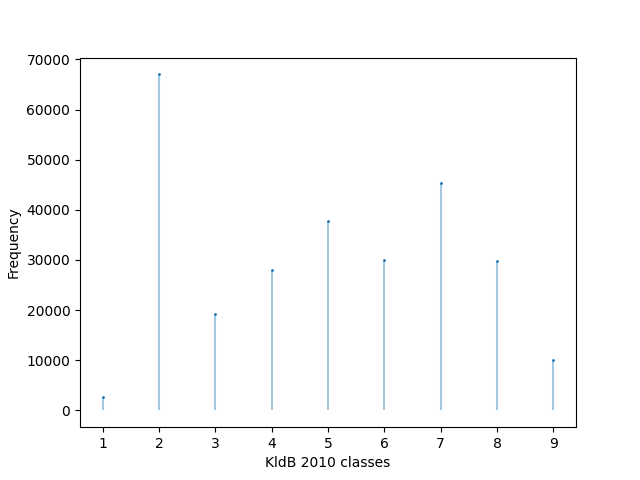
\includegraphics[width=.9\linewidth]{training_data_long_L1.png}
    \caption{\label{fig: F11} Class distribution Level 1}
  \end{subfigure}%
  \begin{subfigure}{.5\textwidth}
    \centering
    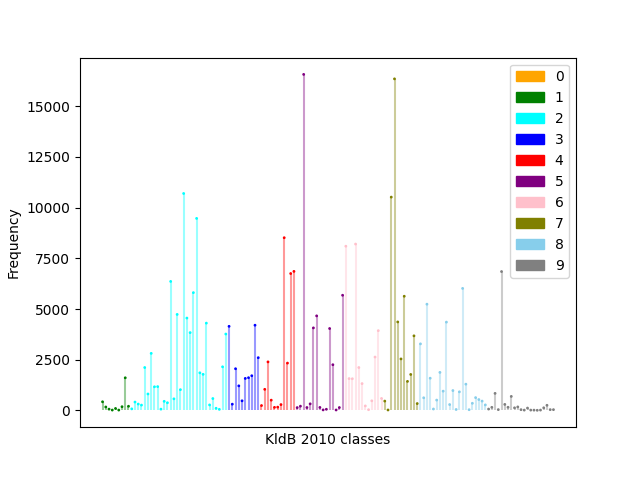
\includegraphics[width=.9\linewidth]{training_data_long_L3.png}
    \caption{\label{fig: F12} Class distribution Level 3}
  \end{subfigure}
  \caption{Class distribution of training data}
  \end{figure}

% \section{Naive Bayes Classifier}
% \subsection{Theory}
% The \ac{NB}, a family of probabilistic classifiers, uses Bayes' rule in order to determine the most likely class for each document \citep{Schneider2005}. All \ac{NB} classifiers rely on the conditional independence assumptions which means, that ``features are independent of each other, given the category variable'' \citep[48]{Xu2018}. Depending on whether the features are discrete or continous, different distributions, so-called event models are proposed. While from a theoretical perspective for continous features Gaussian distribution is well-suited, for discrete features usually Bernoulli or multinomial distibutions are applied \citep{Xu2018}. Although, popular practical implementations, like the one from sklearn, allow as well fractional counts for multinomial distributions \citep{scikit-learn}. Trying different event models, the multinomial \ac{NB} shows indeed for both Count Vectorizer and for TFIDF the best results, which is why I choose it as event model for the baseline. 

% The multinomial \ac{NB} classifies according to the most likely class. Given that a document d has $t = 1, ...., k$ terms and can be assigned to $c = 1,...,j$ classes, the probability of a term in a document given a class is calculated as \citep{Manning2008}:
% \[ P(t_k, c_j) = \frac{occurence(t_k, c_j) + 1}{\sum occurence(t, c_j) + |V|} \]

% where $|V|$ is the cardinality of the vocabulary. In the denominator 1 is added, so-called Laplace smoothing, in order to avoid zeros, which is the case if the number of terms in a document for one class is zero. \citep{Manning2008}. Further given that $N_c = count(c_j)$ is the number of documents belonging to class $c_j$ and N is number of documents the probability of $c_j$ is defined as $\frac{N_c}{N}$. The probability of a document d belonging to a class $c_j$ can then formulated as follows \citep[258]{Manning2008}:
% \[ P(c_j|d) \propto P(c_j) \prod_{i = 1}^k P(t_i|c_j) \]
% Then the most likely classes can be determined by \citep{Manning2008}: 
% \[\argmax_{c \in C} P(c_j) \prod_{i = 1}^k P(t_i|c_j) \] 

\section{Results}

\end{document}